\documentclass[12pt]{article}
\usepackage{amsmath, amssymb, amsfonts, amsthm, mathtools}
\usepackage{thmtools}
\usepackage[utf8]{inputenc}
\usepackage[inline]{enumitem}
\usepackage[colorlinks=true]{hyperref}
\usepackage{tikz-cd}
\usepackage{tikz}
\usetikzlibrary{decorations.markings}
\usetikzlibrary{arrows.meta}
\setlength\parindent{0pt}

\theoremstyle{definition}
\newtheorem{thm}{Theorem}
\numberwithin{thm}{section}
\newtheorem{lem}[thm]{Lemma}
\newtheorem{defn}[thm]{Definition}
\newtheorem{prop}[thm]{Proposition}
\newtheorem{cor}[thm]{Corollary}
\newtheorem{ex}{Example}
\newtheorem{exe}[thm]{Exercise}
% \numberwithin{exe}{section}


\let\emptyset\varnothing
\newcommand{\rel}{\;\;\operatorname{rel}\;}
\newcommand{\id}{\operatorname{id}}

\pagestyle{plain}

% \usepackage{titlesec}
% \titleformat{\section}[block]
%   {\newpage\center\normalfont}{\S\thesection}{0.25cm}{\large}

\usepackage{titlesec}
\titleformat{\section}[block]{\newpage\sffamily\Large\filcenter\bfseries}{\S\thesection.}{0.25cm}{\Large}
\titleformat{\subsection}[block]{\large\bfseries\sffamily}{\S\S\thesubsection.}{0.2cm}{\large}


\usepackage[a4paper]{geometry}
\usepackage{lipsum}

\usepackage{cleveref}
\crefname{thm}{Theorem}{Theorems}
\crefname{lem}{Lemma}{Lemmas}
\crefname{defn}{Definition}{Definitions}
\crefname{prop}{Proposition}{Propositions}
\crefname{cor}{Corollary}{Corollaries}
\crefname{exe}{Exercise}{Exercises}
\crefname{equation}{}{}

\usepackage{mdframed}
\newenvironment{blockquote}
{\begin{mdframed}[skipabove=0pt, skipbelow=0pt, innertopmargin=4pt, innerbottommargin=4pt, bottomline=false,topline=false,rightline=false, linewidth=2pt]}
{\end{mdframed}}
\newenvironment{soln}{\begin{proof}[Solution]}{\end{proof}}

\usepackage{fancyhdr}
\pagestyle{fancy}
\fancyhf{}
\fancyhead[L]{\sffamily{\S\textbf{\nouppercase{\leftmark}}}}
\fancyhead[R]{\sffamily{\thepage}}
% \renewcommand{\headrulewidth}{0pt}

% \renewcommand{\familydefault}{\rmdefault}
% \usepackage{tgtermes}

\usepackage[textwidth=3cm, textsize=small, colorinlistoftodos]{todonotes}
% Rekha's notes
\newcommand{\rsnote}[1]{\todo[color=yellow!20,linecolor=yellow!20!black,size=\tiny]{#1}}
\newcommand{\rsnoteil}[1]{\ \todo[inline,color=yellow!20,linecolor=yellow!40!black,size=\normalsize]{#1}}

% Aryaman's notes
\newcommand{\amnote}[1]{\todo[color=orange!40,linecolor=orange!40!black,size=\tiny]{#1}}
\newcommand{\amnoteil}[1]{\ \todo[inline,color=orange!40,linecolor=orange!40!black,size=\normalsize]{#1}}

\title{Algebraic Topology}
\author{Aryaman Maithani\\\url{https://aryamanmaithani.github.io/}}
% \date{Spring Semester 2019-20}

\begin{document}
\maketitle
\tikzset{lab dis/.store in=\LabDis,
  lab dis=0.3,
  ->-/.style args={at #1 with label #2}{decoration={
    markings,
    mark=at position #1 with {\arrow{>}; \node at (0,\LabDis) {#2};}},postaction={decorate}},
    -<-/.style args={at #1 with label #2}{decoration={
    markings,
    mark=at position #1 with {\arrow{<}; \node at (0,\LabDis)
    {#2};}},postaction={decorate}},
   -*-/.style={decoration={
    markings,
    mark=at position #1 with {\fill (0,0) circle (1.5pt);}},postaction={decorate}},
  }
In what follows, $I$ will denote the closed interval $[0, 1] \subset \mathbb{R}.$\\
Whenever we talk about a map $f:X\to Y$ between topological spaces $X$ and $Y,$ we will always mean a \emph{continuous function} $f.$\\
A path $\sigma$ in a space $X$ is a map $\sigma: I \to X.$ If $x_0 = \sigma(0)$ and $x_1 = \sigma(1),$ we write this as
\begin{equation*} 
	x_0 \overset{\sigma}{\longrightarrow} x_1.
\end{equation*}
Moreover, $x_0$ and $x_1$ are called the \emph{end points} of $\sigma.$ In particular, $x_0$ is the initial point and $x_1$ is the terminal point.\\
All the topological spaces are assumed to be nonempty.\\
\begin{thm}[The Eckmann-Hilton Argument] \label{thm:eckmannhilton}
	Let $M$ be a set and $*, \star$ be two unital binary operations on $M$ with units $1_*$ and $1_\star,$ respectively. Suppose that
	\begin{equation*} 
		(a * b) \star (c * d) = (a \star c) * (b \star d)
	\end{equation*}
	for all $a, b, c, d \in M.$\\
	Then, $1_* = 1_\star,$ $* = \star,$ and furthermore, the operation(s) are commutative and associative.
\end{thm}
\begin{proof} \phantom{hi}\\
	\textbf{Claim 1.} $1_* = 1_\star.$
	\begin{align*} 
		1_* = 1_* * 1_* &= (1_* \star 1_\star) * (1_\star \star 1_*)\\
		&=(1_* * 1_\star) \star (1_\star * 1_*) = 1_\star \star 1_\star = 1_\star.
	\end{align*}
	Thus, we define $1 \vcentcolon= 1_* = 1_\star$ which is the unit for both operations.

	\dotfill

	\textbf{Claim 2.} $a*b = a\star b$ for all $a, b \in M.$
	\begin{align*} 
		a * b &= (a \star 1) * (1 \star b)\\
		&= (a * 1) \star (1 * b) = a \star b.
	\end{align*}
	Thus, we define $\cdot = * = \star.$

	\dotfill

	\textbf{Claim 3.} $a\cdot b = b\cdot a$ for all $a, b \in M.$
	\begin{align*} 
		a \cdot b &= (1 \cdot a) \cdot (b \cdot 1)\\
		&= (1 \cdot b) \cdot (a \cdot 1) = b \cdot a.
	\end{align*}

	\dotfill

	\textbf{Claim 4.} $(a\cdot b) \cdot c = a\cdot(b\cdot c)$ for all $a, b, c \in M.$
	\begin{align*} 
		(a\cdot b) \cdot c &= (a\cdot b) \cdot (1 \cdot c)\\
		&= (a\cdot 1) \cdot (b \cdot c) = a \cdot (b \cdot c).
	\end{align*}

	Thus, we have proven all the claims.
\end{proof}
\section{Homotopy of Paths}
%
\subsection{The Fundamental Group}

\begin{defn}[Homotopy]
	Let $\sigma$ and $\tau$ be paths in a space $X$ with the same end points, i.e., $\sigma(0) = \tau(0)$ and $\sigma(1) = \tau(1).$\\
	We say that $\sigma$ and $\tau$ are \emph{homotopic with ends points held fixed} written
	\begin{equation*} 
		\sigma \simeq \tau \rel \{0, 1\}
	\end{equation*}
	if there is a map $F: I \times I \to X$ such that
	\begin{enumerate}
		\item $F(s, 0) = \sigma(s)$ for all $s \in I,$
		\item $F(s, 1) = \tau(s)$ for all $s \in I,$
		\item $F(0, t) = x_0$ for all $t \in I,$
		\item $F(1, t) = x_1$ for all $t \in I.$
	\end{enumerate}
	$F$ is called a \emph{homotopy} from $\sigma$ to $\tau.$ We write
	\begin{equation*} 
		F : \sigma \simeq \tau \rel \{0, 1\}.
	\end{equation*}
\end{defn}
The above can be pictorially depicted as

\begin{center}
	\begin{tikzpicture}
		\def \len{2.5}
		\draw[thick, ->-=at 0.5 with label {$x_0$}](0, 0) -- (0, \len);
		\draw[thick, ->-=at 0.5 with label {$\tau$}](0, \len) -- (\len, \len);
		\draw[thick, -<-=at 0.5 with label {$x_1$}](\len, \len) -- (\len, 0);
		\draw[thick, -<-=at 0.5 with label {$\sigma$}](\len, 0) -- (0, 0);
	\end{tikzpicture}
\end{center}

The above picture is interpreted as follows: \\
Along the (bottom) line $t = 0,$ $F$ agrees with $\sigma$ and along the (top) line $t = 1,$ $F$ agrees with $t = 1.$\\
Similarly, along the (left) line $s = 0,$ $F$ is identically equal to $x_0$ and along the (right) line $s = 1,$ it is $x_1.$\\~\\
%
In particular, if $\sigma$ is a \emph{loop}, i.e., $x_0 = x_1$ and $e_{x_0}$ is the constant loop $s \mapsto x_0$ for $s \in I,$ and if $\sigma \simeq e_{x_0} \rel \{0, 1\},$ we say that ``$\sigma$ can be shrunk to a point,'' or is \emph{homotopically trivial}.

\begin{prop}[$\simeq$ is an equivalence relation] \label{prop:equivrel}
	\phantom{hi}\\
	\begin{enumerate}
		\item $\sigma \simeq \sigma \rel \{0, 1\},$
		\item $\sigma \simeq \tau \rel \{0, 1\} \implies \tau \simeq \sigma \rel \{0, 1\},$
		\item $\sigma \simeq \tau \rel \{0, 1\}$ and $\tau \simeq \rho \rel \{0, 1\} \implies \sigma \simeq \rho \rel \{0, 1\}.$ 
	\end{enumerate}
\end{prop}
\begin{proof} 
	\begin{enumerate}
		\item Define $F(s, t) \vcentcolon= \sigma(s).$
		\item Define $F(s, t) \vcentcolon= F(s, 1 - t).$
		\item Given $F:\sigma \simeq \tau \rel \{0, 1\}$ and $G:\tau \simeq \rho \rel \{0, 1\},$ define $H:I \times I \to X$ as

		\begin{equation*} 
			H(s, t) \vcentcolon= \begin{cases}
				F(s, 2t) & 0 \le 2t \le 1,\\
				G(s, 2t - 1) & 1 \le 2t \le 2.
			\end{cases}
		\end{equation*}
		Note that $F$ and $G$ do agree for $2t = 1$ since we have $F(s, 1) = \tau(s) = G(s, 0)$ for all $s \in I.$ It is easy to see that $H$ is well-defined.\\
		Note that $H$ is continuous (by the pasting lemma) and it satisfies all the four properties of a homotopy (from $\sigma$ to $\rho$), since $F$ and $G$ do so. \qedhere
	\end{enumerate}
\end{proof}
Thus, we can consider the homotopy classes $[\sigma]$ of paths $\sigma$ from $x_0$ to $x_1$ under the equivalence relation $\simeq.$ (Note very carefully that all paths in an equivalence class have the same end points.)

\begin{defn}[Multiplication of paths]
	Let $\sigma$ be a path from $x_0$ to $x_1$ and $\tau$ from $x_1$ to $x_2.$\\
	The product $\sigma*\tau$ is a path from $x_0$ to $x_2$ defined as
	\begin{equation*} 
		\sigma*\tau(s) \vcentcolon= \begin{cases}
			\sigma(2s) & 0 \le 2s \le 1,\\
			\tau(2s - 1) & 1 \le 2s \le 2.
		\end{cases}
	\end{equation*}
	Once again, it's an easy check that $\sigma\tau$ is well-defined and continuous (using the pasting lemma).
\end{defn}

The above $\sigma*\tau$ is essentially the path from $x_0$ to $x_1$ obtained by first travelling from $x_0$ to $x_1$ via $\sigma$ and then from $x_1$ to $x_2$ via $\tau.$\\~\\
We will now be lenient with notation and simply denote $\sigma*\tau$ as $\sigma\tau$ unless necessary.\\
The next proposition shows how this product behaves with the equivalence relation.

\begin{prop}
	\begin{equation*} 
		\sigma \simeq \sigma' \rel \{0, 1\} \text{ and } \tau \simeq \tau' \rel \{0, 1\} \implies \sigma\tau \simeq \sigma'\tau' \rel \{0, 1\}.
	\end{equation*}
\end{prop}
\begin{proof} 
	The proof is motivated by the following diagram.\\
	\begin{center}
		\begin{tikzpicture}
			\def \len{3}
			\draw[thick, ->-=at 0.5 with label {$x_0$}](0, 0) -- (0, \len);
			\draw[thick, ->-=at 0.5 with label {$\sigma'$}](0, \len) -- (\len, \len);
			\draw[dashed, -<-=at 0.5 with label {$x_1$}, -*-=at 0.0 with label {}, -*-=at 1.0 with label {}](\len, \len) -- (\len, 0);
			\draw[thick, -<-=at 0.5 with label {$\sigma$}](\len, 0) -- (0, 0);
			\draw[thick, ->-=at 0.5 with label {$\tau'$}](\len, \len) -- (2*\len, \len);
			\draw[thick, -<-=at 0.5 with label {$x_2$}](2*\len, \len) -- (2*\len, 0);
			\draw[thick, -<-=at 0.5 with label {$\tau$}](2*\len, 0) -- (\len, 0);
			\node[] at (\len/2, \len/2) {$F$};
			\node[] at (3*\len/2, \len/2) {$G$};
		\end{tikzpicture}
	\end{center}

	Given $F:\sigma \simeq \sigma' \rel \{0, 1\}$ and $G:\tau \simeq \tau' \rel \{0, 1\},$ define $H:I \times I \to X$ as

	\begin{equation*} 
		H(s, t)\vcentcolon= \begin{cases}
				F(2s, t) & 0 \le 2s \le 1,\\
				G(2s - 1, t) & 1 \le 2s \le 2.
			\end{cases}
	\end{equation*}

	As earlier, $H$ is well-defined (since $F(1, t) = x_1 = G(0, t)$ for all $t \in I$) and continuous. Moreover, we have
	\begin{equation*} 
		H(0, t) = F(0, t) = x_0, \quad H(1, t) = G(1, t) = x_2,
	\end{equation*}
	\begin{equation*} 
		H(s, 0)= \begin{cases}
				F(2s, 0) & 0 \le 2s \le 1,\\
				G(2s - 1, 0) & 1 \le 2s \le 2
			\end{cases} = \begin{cases}
				\sigma(2s) & 0 \le 2s \le 1,\\
				\tau(2s - 1) & 1 \le 2s \le 2
			\end{cases} = \sigma\tau(s),
	\end{equation*}
	and similarly, 
	\begin{equation*} 
		H(s, 1) = \sigma'\tau'(s)\text{ for all }s \in I.
	\end{equation*}\\
	This shows that 
	\begin{equation*} 
		H : \sigma\tau\simeq\sigma'\tau' \rel \{0, 1\}. \qedhere
	\end{equation*}
\end{proof}
\begin{defn}[Product of equivalence classes]
	In view of the above proposition, we define
	\begin{equation*} 
		[\sigma]*[\tau] \vcentcolon= [\sigma*\tau].
	\end{equation*}
\end{defn}
The above, of course, is defined only when the terminal point of $\sigma$ (and thus, any other representative of $[\sigma]$) equals the initial point of $\tau$ (and thus, any other representative of $[\tau]$).\\
As before, we shall drop the $*$ and simply write $[\sigma][\tau].$

\begin{lem} \label{lem:prodassoc}
	Let $\sigma, \tau, \omega$ be paths such that the products $\sigma(\tau\omega)$ and $(\sigma\tau)\omega$ are defined. Then,
	\begin{equation*} 
		\sigma(\tau\omega) \simeq (\sigma\tau)\omega \rel \{0, 1\}.
	\end{equation*}
\end{lem}
\begin{proof} 
	Let $x_0, x_1, x_2, x_3$ be points such that
	\begin{equation*} 
		x_0 \overset{\sigma}{\longrightarrow} x_1 \overset{\tau}{\longrightarrow} x_2 \overset{\omega}{\longrightarrow} x_3. 
	\end{equation*}
	We define a homotopy $F$ from $\sigma(\tau\omega)$ to $(\sigma\tau)\omega.$ To motivate the definition of $F,$ we may first visualise the homotopy as follows.
	\begin{center}
		\begin{tikzpicture}
			\def\len{2}
			\def\height{3}
	\draw[thick, ->-=at 0.5 with label {$x_0$}](0, 0) -- (0, \height);
	\draw[thick, ->-=at 0.5 with label {$\sigma$}](0, \height) -- (\len, \height);
	\draw[thick, ->-=at 0.5 with label {$\tau$}](\len, \height) -- (2*\len, \height);
	\draw[thick, ->-=at 0.5 with label {$\omega$}](2*\len, \height) -- (4*\len, \height);
	\draw[thick, -<-=at 0.5 with label {$x_3$}](4*\len, \height) -- (4*\len, 0);
	\draw[thick, -<-=at 0.5 with label {$\omega$}](4*\len, 0) -- (3*\len, 0);
	\draw[thick, -<-=at 0.5 with label {$\tau$}](3*\len, 0) -- (2*\len, 0);
	\draw[thick, -<-=at 0.5 with label {$\sigma$}](2*\len, 0) -- (0, 0);
	\draw[dashed,-*-=at 0.0 with label {},-*-=at 1.0 with label {}](\len, \height) -- (2*\len, 0);
	\draw[dashed, -*-=at 0.0 with label {}, -*-=at 1.0 with label {}](2*\len, \height) -- (3*\len, 0);
		\end{tikzpicture}
	\end{center}
	One can note that the top line depicts the path $(\sigma\tau)\omega$ and the bottom $\sigma(\tau\omega).$\\~\\
	We define $F:I \times I \to X$ piece-wise on the three regions (from left to right) as follows:

	\begin{equation*} 
		F(s, t) \vcentcolon= \begin{cases}
			\sigma\left(\dfrac{4s}{2 - t}\right) & 0 \le s \le \dfrac{1}{4}(2 - t) ,\\~\\
			\tau\left(4s + 2 - t\right) & \dfrac{1}{4}(2 - t) \le s \le \dfrac{1}{4}(3 - t),\\~\\
			\omega\left(\dfrac{4s + t - 3}{t + 1}\right) & \dfrac{1}{4}(3 - t) \le s \le 1.
		\end{cases}
	\end{equation*}
	It is clear that $F$ is continuous on each piece. By the pasting lemma, it is continuous everywhere.\\
	The four properties of being a homotopy are also clear, by construction. (The diagram makes it clear why.)
\end{proof}

\begin{defn}[Inverse path]
	Given a path $\sigma$ from $x_0$ to $x_1,$ its \emph{inverse path} $\sigma^{-1}$ is a path from $x_1$ to $x_0$ given by
	\begin{equation*} 
		\sigma^{-1}(s) \vcentcolon= \sigma(1 - s), \qquad s \in I.
	\end{equation*}
\end{defn}
The above is simply ``travelling backwards $\sigma$.''
\begin{lem} 
	Let $\sigma, \sigma':I \to X$ be paths such that $\sigma \simeq \sigma' \rel \{0, 1\}.$ Then,
	\begin{equation*} 
		\sigma^{-1} \simeq \sigma'^{-1} \rel \{0, 1\}.
	\end{equation*}
\end{lem}
\begin{proof} 
	Let $F:\sigma \simeq \sigma' \rel \{0, 1\}$ be a homotopy. Then, $F'(s, t) \vcentcolon= F(1 - s, t)$ is a homotopy between the inverses.
\end{proof}

\begin{defn}[Inverse class]
	Let $\sigma:I \to X$ be a path. We define the inverse of the class $[\sigma]$ as
	\begin{equation*} 
		[\sigma]^{-1} \vcentcolon= [\sigma^{-1}].
	\end{equation*}
\end{defn}
In view of the above lemma, the above definition is indeed well-defined.

\begin{lem} \label{lem:prodinv}
	Given any path $\sigma$ from $x_0$ to $x_1,$ we have
	\begin{equation*} 
		e_{x_0} \simeq \sigma\sigma^{-1} \rel \{0, 1\},
	\end{equation*}
	where $e_{x_0}$ denotes the constant loop at $x_0.$
\end{lem}

\begin{proof} 
	As usual, we motivate the proof with a diagram. In this case, it is the following:
	\begin{center}
		\begin{tikzpicture}
			\def\len{3}
			\draw[thick, ->-=at 0.5 with label {$x_0$}](0, 0) -- (0, \len);
			\draw[thick, ->-=at 0.5 with label {$\sigma$}](0, \len) -- (\len, \len);
			\draw[thick, -<-=at 0.5 with label {$e_{x_0}$}](2*\len, 0) -- (0, 0);
			\draw[thick, ->-=at 0.5 with label {$\sigma^{-1}$}](\len, \len) -- (2*\len, \len);
			\draw[thick, -<-=at 0.5 with label {$x_0$}](2*\len, \len) -- (2*\len, 0);
			\draw[dashed, -*-=at 0.5 with label {$x_1$}] (0, 0) -- (\len, \len) -- (2*\len, 0);
		\end{tikzpicture}
	\end{center}
	The homotopy $F:I \times I \to X$ in this case, is defined as
	\begin{equation*} 
		F(s, t) \vcentcolon= \begin{cases}
			\sigma(2s) & 0 \le 2s \le t,\\
			\sigma(t) & t \le 2s \le 2 - t,\\
			\sigma^{-1}(2s - 1) & 2 - t \le 2s \le 2.
		\end{cases}
	\end{equation*}
	It is clear that the piecewise definitions agree on the dashed line $2s = t.$ Observe that $\sigma^{-1}(2s - 1) = \sigma(2 - 2s)$ and thus, the functions do agree on the dashed line $2s = 2 - t$ as well. \\
	One can easily check that the four properties of the homotopy are satisfied. To see the bottom line property, note that $F(s, 0) = \sigma(0)$ (using the second piece definition) and $\sigma(0) = x_0 = e_{x_0}(s)$ for all $s \in I.$
\end{proof}

Note that since $(\sigma^{-1})^{-1} = \sigma,$ the above also shows that $\sigma^{-1}\sigma = e_{x_1}.$

\begin{lem} \label{lem:leftid}
	Let $x_0 \overset{\sigma}{\longrightarrow} x_1$ and $e_{x_0}$ be the constant path at $x_0.$ Then,
	\begin{equation*} 
		\sigma \simeq e_{x_0}\sigma \rel \{0, 1\}.
	\end{equation*}
\end{lem}
\begin{proof} 
	The proof is motivated by this diagram.

	\begin{center}
		\begin{tikzpicture}
			\def\len{3}
			\draw[thick, ->-=at 0.5 with label {$x_0$}](0, 0) -- (0, \len);
			\draw[thick, ->-=at 0.5 with label {$e_{x_0}$}](0, \len) -- (\len, \len);
			\draw[thick, -<-=at 0.5 with label {$\sigma$}](2*\len, 0) -- (0, 0);
			\draw[thick, ->-=at 0.5 with label {$\sigma$}](\len, \len) -- (2*\len, \len);
			\draw[thick, -<-=at 0.5 with label {$x_1$}](2*\len, \len) -- (2*\len, 0);
			\draw[dashed, -*-=at 1.0 with label {$x_0$}] (0, 0) -- (\len, \len);
		\end{tikzpicture}
	\end{center}

	The homotopy is $F:I\times I \to X$ defined as
	\begin{equation*} 
		F(s, t) \vcentcolon= \begin{cases}
			x_0 & 0 \le 2s \le t,\\~\\
			\sigma\left(\dfrac{2s - t}{2 - t}\right) & t \le 2s \le 2.
		\end{cases}
		\qedhere
	\end{equation*}
\end{proof}

As one would expect, we have a lemma in the other direction as well.
\begin{lem} \label{lem:rightid}
	Let $x_1 \overset{\sigma}{\longrightarrow} x_0$ and $e_{x_0}$ be the constant path at $x_0.$ Then,
	\begin{equation*} 
		\sigma \simeq \sigma e_{x_0} \rel \{0, 1\}.
	\end{equation*}
\end{lem}

\begin{proof} 
	Similar as in the last case and we omit it.
\end{proof}
	
The astute reader might have sensed a group sneaking around the corner.\\
However, note that the product of equivalence classes defined above is not a binary operation unless the endpoints are the same. Due to this, we restrict ourselves to loops in the next theorem.

\begin{thm}
	Let $\pi_1(X, x_0)$ be the set of homotopy classes of loops in $X$ at $x_0.$\\
	If multiplication in $\pi_1(X, x_0)$ is defined as above, $\pi_1(X, x_0)$ becomes a group, in which the neutral element is the class $[e_{x_0}]$ and the inverse of a class $[\sigma]$ is the class of the inverse $[\sigma^{-1}].$
\end{thm}
\begin{proof} 
	Interpreting \crefrange{lem:prodassoc}{lem:rightid} as equalities of the equivalence classes shows that $\pi_1(X, x_0)$ verifies the group axioms.
\end{proof}

The next proposition tells us how $\pi_1(X, x_0)$ and $\pi_1(X, x_1)$ are related in the case that $x_0$ and $x_1$ lie in the same path-connected component. (In the case that they do not, nothing can be said.)

\begin{prop}
	Let $\alpha$ be a path from $x_0$ to $x_1.$ The mapping $\widehat{\alpha}$ defined by
	\begin{equation*} 
		[\sigma] \mapsto [\alpha^{-1}]*[\sigma]*[\alpha] = [\alpha^{-1}\sigma\alpha]
	\end{equation*}
	is an isomorphism of the group $\pi_1(X, x_0)$ onto $\pi_1(X, x_1).$
\end{prop}
Note that the above is well-defined since $*$ is well-defined.
\begin{proof} 
	We first note that if $[\sigma] \in \pi_1(X, x_0),$ then $\alpha^{-1}\sigma\alpha$ is path as follows:
	\begin{equation*} 
		x_1 \overset{\alpha^{-1}}{\longrightarrow} x_0 \overset{\sigma}{\longrightarrow} x_0 \overset{\alpha}{\longrightarrow} x_1
	\end{equation*}
	and thus, $[\alpha^{-1}\sigma\alpha]$ is indeed an element of $\pi_1(X, x_1).$\\
	Moreover, note that
	\begin{align*} 
		\widehat{\alpha}([\sigma\sigma']) &= [\alpha^{-1}\sigma\sigma'\alpha]\\
		&= [\alpha^{-1}\sigma][\sigma'\alpha]\\
		&= [\alpha^{-1}\sigma][\alpha\alpha^{-1}][\sigma'\alpha]\\
		&= [\alpha^{-1}\sigma\alpha][\alpha^{-1}\sigma'\alpha]\\
		&= \widehat{\alpha}([\sigma])\widehat{\alpha}([\sigma']).
	\end{align*}
	This shows that $\widehat{\alpha}$ is a homomorphism. That this is an isomorphism follows by noting that it has as inverse $\widehat{\alpha^{-1}}.$
\end{proof}
\begin{cor}
	If $X$ is path-connected, the group $\pi_1(X, x_0)$ is independent of the point $x_0,$ up to isomorphism.
\end{cor}
Note that if $C$ is a connected component of $X$ containing $x_0,$ then $\pi_1(X, x_0) = \pi_1(C, x_0)$ since any loop at $x_0$ must necessarily lie in $C.$ For this reason, we might as well only work with path-connected spaces.
\begin{defn}
	If $X$ is path-connected, we write $\pi_1(X)$ for $\pi_1(X, x_0)$ and call it \emph{the fundamental group} of $X.$
\end{defn}
Note that this group depends on $x_0$ in the sense that the elements of the group depend on the base point $x_0$ but the isomorphism class does not.\\
\begin{defn}[Simply connected]
	A space $X$ is called simply connected if it is path-connected and its fundamental group is trivial.
\end{defn}
\begin{lem} \label{lem:simpconnpathshomot}
	Let $X$ be simply connected. If $\sigma$ and $\tau$ are paths in $X$ with the same initial and terminal points, then $\sigma \simeq \tau \rel \{0, 1\}.$
\end{lem}
\begin{proof} 
	Let the initial and terminal points be $x_0$ and $x_1,$ respectively.\\
	Consider the path $\sigma\tau^{-1},$ which is path at $x_0.$ Since $X$ is simply connected, we have
	\begin{equation*} 
		\sigma\tau^{-1} \simeq e_{x_0} \rel \{0, 1\}.
	\end{equation*}
	By the previously seen properties, we see that
	\begin{equation*} 
		(\sigma\tau^{-1})\tau \simeq e_{x_0}\tau \rel \{0, 1\}
	\end{equation*}
	or
	\begin{equation*} 
		\sigma \simeq \tau \rel \{0, 1\}. \qedhere
	\end{equation*}
\end{proof}
\subsection{Functoriality}
We now wish to turn $\pi_1$ into a functor. Since we need to take care of the base points, we look at the category of \emph{Pointed Topological spaces}.
\begin{defn}[Pointed Topological Spaces]
	The category $\mathsf{Top}_\bullet$ of \emph{pointed topological spaces} is the category whose objects and morphisms are given as follows:
	\begin{itemize}
		\item Objects: Pairs $(X, x_0)$ where $X$ is a topological space and $x_0 \in X,$
		\item Morphisms: $f:(X, x_0) \to (Y, y_0)$ such that $f:X\to Y$ is a continuous function and $f(x_0) = y_0.$
	\end{itemize}
\end{defn}
That the above is a category can be easily verified.

\begin{defn}
	Let $h:(X, x_0) \to (Y, y_0)$ be a morphism. Define
	\begin{equation*} 
		h_* : \pi_1(X, x_0) \to \pi_1(Y, y_0)
	\end{equation*}
	by the equation
	\begin{equation*} 
		h_*([\sigma]) = [h\circ \sigma].
	\end{equation*}
	The map $h_*$ is called the \emph{homomorphism induced by $h$}, relative to the base point $x_0.$
\end{defn}
To see that $h_*$ is well-defined, we note that if 
\begin{equation*} 
	F : \sigma \simeq \sigma' \rel \{0, 1\}
\end{equation*}
for loops $\sigma, \sigma'$ in $X$ at $x_0,$ then
\begin{equation*} 
	h \circ F : h\circ \sigma \simeq h\circ\sigma' \rel \{0, 1\}.
\end{equation*}
That is to say, if two loops at $x_0$ are homotopic, then so are the loops obtained by pre-composing $h.$\\~\\
To see that $h_*$ is a homomorphism, first note that
\begin{equation*} 
	(h \circ \sigma)(h \circ \sigma') = h\circ(\sigma\sigma').
\end{equation*}
(This follows from the definition of the product of paths.)\\
Then, we see that
\begin{equation*} 
	h_*([\sigma\sigma']) = [h\circ(\sigma\sigma')] = [h\circ\sigma][h\circ\sigma'] = h_*([\sigma])h_*([\sigma']).
\end{equation*}

\begin{thm}[Functoriality]
	If $h:(X, x_0) \to (Y, y_0)$ and $k:(Y, y_0) \to (Z, z_0)$ are morphisms, then
	\begin{equation*} 
		(k \circ h)_* = k_* \circ h_*.
	\end{equation*}
	If $i:(X, x_0) \to (X, x_0)$ is the identity map, then $i_*$ is the identity homomorphism.
\end{thm}
\begin{proof} 
	By definition, we have
	\begin{align*} 
		(k \circ h)_*([\sigma]) &= [(k \circ h) \circ \sigma]\\
		&= [k \circ (h \circ \sigma)]\\
		&= k_*([h\circ \sigma])\\
		&= k_*(h_*([\sigma]))\\
		&= (k_* \circ h_*)([\sigma]).
	\end{align*}
	Thus, $(k \circ h)_* = k_* \circ h_*.$\\~\\
	Now, if $i$ is the identity map, then we have
	\begin{equation*} 
		i_*([\sigma]) = [i \circ \sigma] = [\sigma],
	\end{equation*}
	showing that $i_*$ is the identity map of $\pi_1(X, x_0).$
\end{proof}
The above then shows that $\pi_1$ defines a functor from the category $\mathsf{Top}_*$ to $\mathsf{Grp}.$\\
Since functors preserve isomorphisms in general, we get the following corollary.
\begin{cor}
	If $h:(X, x_0) \to (Y, y_0)$ is a morphism such that $h:X \to Y$ is a homeomorphism, then
	\begin{equation*} 
		h_* : \pi_1(X, x_0) \to \pi_1(Y, y_0)
	\end{equation*}
	is an isomorphism.
\end{cor}
Since we aren't discussing Category Theory, we give a proof for this special example of functors.
\begin{proof} 
	Let $h^{-1}:Y \to X$ be the inverse, which is continuous since $h$ is a homeomorphism. Moreover, $h^{-1}(y_0) = x_0$ and thus, $h^{-1}:(Y, y_0) \to (X, x_0)$ is a morphism and the inverse of $h.$\\
	Now, note that,
	\begin{equation*} 
		(h_*)\circ((h^{-1})^*) = (h\circ h^{-1})^* = (\id_{(Y, y_0)})^* = \id_{\pi_1(Y, y_0)},
	\end{equation*}
	by functoriality. Similarly, we have
	\begin{equation*} 
		((h^{-1})^*)\circ(h_*) = \id_{(X, x_0)},
	\end{equation*}
	proving the corollary.
\end{proof}
%
%
\section{Homotopy of Maps}
%
In the previous section, we talked about homotopy of special types of maps. More precisely, we only considered maps $I \to X.$ However, we can replace $I$ by an arbitrary topological space $Y.$ In the place of endpoints, we just consider a subspace $A \subset Y.$
\begin{defn}[Relative homotopy]
	Given maps $f, g:Y \to X$ such that $f|_A = g|_A,$ we say $f$ and $g$ are homotopic relative to $A$ written
	\begin{equation*} 
		f \simeq g \rel A
	\end{equation*}
	if there is a map $F:Y \times I \to X$ satisfying
	\begin{enumerate}
		\item $F(y, 0) = f(y)$ for all $y \in Y,$
		\item $F(y, 1) = g(y)$ for all $y \in Y,$
		\item $F(a, t) = f(a) = g(a)$ for all $a \in A, t \in I.$
	\end{enumerate}
	This map $F$ is called a homotopy from $f$ to $g$ relative to $A$ and we write
	\begin{equation*} 
		F:f\simeq g \rel A.
	\end{equation*}
\end{defn}
Note that the ``second coordinate'' above is still $I.$\\
Note that (3) is satisfied vacuously if $A = \emptyset$ and we have $f|_A = g|_A$ for all maps $f, g : Y \to X.$ Keeping this in mind, we have the following definition.
\begin{defn}[Homotopy]
	Maps $f, g:Y \to X$ are said to be \emph{homotopic} if $f$ and $g$ are homotopic relative to $\emptyset.$\\
	We write this more simply as
	\begin{equation*} 
		f \simeq g.
	\end{equation*}
	Moreover, any $F$ as before is simply called a homotopy from $f$ to $g.$\\
	As before, we write
	\begin{equation*} 
		F:f\simeq g.
	\end{equation*}
\end{defn}

Once again, we obtain an equivalence. The homotopies defined as in the proof of \cref{prop:equivrel} work again.
\begin{defn}[Contractible space] \label{def:contrac}
	If $X$ is a topological space such that the identity map on $X$ is homotopic to a constant map on some point in $X,$ we say that $X$ is \emph{contractible}.
\end{defn}

\begin{prop} \label{prop:contracpath} % ex 3.1
	$X$ is contractible if and only if for any space $Y,$ any two maps of $Y$ into $X$ are homotopic. A contractible space is path-connected.
\end{prop}
\begin{proof} 
	$(\implies)$ Let $X$ be contractible and $Y$ be any space. Fix any $x_0 \in X$ such that $\id_X$ is homotopic to the constant map $e_{x_0}:X\to X.$ \\
	Let $f_{x_0}:Y\to X$ denote the constant map $y \mapsto x_0.$\\
	Now, given any map $f:Y\to X,$ we show that it is homotopic to $f_{x_0}.$ \\This will prove that any two maps of $Y$ into $X$ are homotopic since $\simeq$ is an equivalence relation.\\
	Let $H:\id_X \simeq e_{x_0}$ be any homotopy. Then, we have
	\begin{equation*} 
		H(x, 0) = x,\quad H(x, 1) = x_0; \qquad \text{for all } x \in X.
	\end{equation*}
	(Note that $H$ is continuous.)\\
	Now, we define $F:Y\times I \to X$ as
	\begin{equation*} 
		F(y, t) = H(f(y), t).
	\end{equation*}
	It is clear that $F$ is a map. (That is, $F$ is continuous.)\\
	Moreover, note that
	\begin{equation*} 
		F(y, 0) = H(f(y), 0) = f(y), \quad F(y, 1) = H(f(y), 1) = x_0 = f_{x_0}(y); \qquad \text{for all } y \in Y.
	\end{equation*}
	This shows that $F:f\simeq f_{x_0},$ as desired.\\~\\
	$(\impliedby)$ To show that $X$ is contractible, simply consider $Y = X$ and consider the maps $\id_X$ and $e_{x_0}.$ (Both of these are indeed continuous.)\\
	By hypothesis, these maps are homotopic and by definition, $X$ is contractible.\\~\\
	Now, we show that $X$ is path-connected assuming that it is contractible.\\
	Let $x_0$ and $x_1$ be any two points in $X.$ As $X$ is contractible, $(\implies)$ tells us that the maps $e_{x_0}$ and $e_{x_1}$ are homotopic. \\
	Let $F$ be any homotopy from $e_{x_0}$ and $e_{x_1}.$ Define $\sigma:I\to X$ as 
	\begin{equation*} 
		\sigma(t) \vcentcolon= F(x_0, t).
	\end{equation*}
	$\sigma$ is clearly continuous. Moreover, we have
	\begin{align*} 
		\sigma(0) &= F(x_0, 0) = e_{x_0}(x_0) = x_0,\\
		\sigma(1) &= F(x_0, 1) = e_{x_1}(x_0) = x_1.
	\end{align*}
	Thus, $\sigma$ is path from $x_0$ to $x_1$ in $X,$ proving the proposition.
\end{proof}
\begin{ex}
	Every convex subset $X$ of Euclidean space is contractible.\\
	Given maps $f_1, f_2: Y \to X,$ we have a homotopy $F:f_1 \simeq f_2$ given by
	\begin{equation*} 
		F(y, t) = tf_2(y) + (1 - t)f_1(y), \quad y \in Y, t \in I.
	\end{equation*}
	By the convexity assumption, the above $F$ is indeed a map into $X.$\\
	By the previous proposition, this shows that $X$ is contractible.
\end{ex}
\begin{ex}
	$\mathbb{R}^n$ is contractible for any $n.$\\
	To see this, we could either appeal to the previous example or do it directly by defining a homotopy $F: e_{0} \simeq \id_{\mathbb{R}^n}$ as
	\begin{equation*} 
		F(x, t) = tx.
	\end{equation*}
\end{ex}

We would now like to show that any contractible space is simply connected. What we do know is that any loop would be homotopic to a point. However, we do not know if this homotopy is relative to $\{0, 1\}.$ Indeed, to show that we do have a homotopy relative to $\{0, 1\},$ we would need to use the fact that $X$ is contractible once again.\\
Before proving that, we first look at a lemma.

\begin{lem} \label{lem:gbad}
	Let $F:I\times I \to X$ be a map. Set $\alpha(t) = F(0, t),$ $\beta(t) = F(1, t),$ $\gamma(s) = F(s, 0),$ and $\delta(s) = F(s, 1),$ as in the diagram
	\begin{center}
		\begin{tikzpicture}
			\def \len{3}
			\draw[thick, ->-=at 0.5 with label {$\alpha$}](0, 0) -- (0, \len);
			\draw[thick, ->-=at 0.5 with label {$\delta$}](0, \len) -- (\len, \len);
			\draw[thick, -<-=at 0.5 with label {$\beta$}](\len, \len) -- (\len, 0);
			\draw[thick, -<-=at 0.5 with label {$\gamma$}](\len, 0) -- (0, 0);
			\node[] at (\len/2, \len/2) {$F$};
		\end{tikzpicture}
	\end{center}
	Then, $\delta = \alpha^{-1}\gamma\beta.$
\end{lem}
\begin{proof} 
	The proof is quite intuitive. First, we define the paths
	\begin{equation*} 
		\sigma:I \to I\times I, \quad \tau:I \to I \times I
	\end{equation*}
	as
	\begin{equation*} 
		\sigma(s) \vcentcolon= (t, 1)
	\end{equation*}
	and
	\begin{equation*} 
		\tau(s) \vcentcolon= \begin{cases}
			(0, 1 - 4s) & 0 \le 4s \le 1, \\
			(4s - 1, 0) & 1 \le 4s \le 2, \\
			(1, 2s - 1) & 1 \le 2s \le 2.
		\end{cases}
	\end{equation*}
	These paths are the following ones in $I^2:$
	\begin{center}
		\begin{tikzpicture}
			\def \len{3}
			\draw[thick, ->-=at 0.5 with label {$\sigma$}](0, \len) -- (\len, \len);
			\draw[red, thick, -<-=at 0.5 with label {}](0, 0) -- (0, \len);
			\draw[red, thick, -<-=at 0.5 with label {}](\len, \len) -- (\len, 0);
			\draw[red, thick, -<-=at 0.5 with label {$\tau$}](\len, 0) -- (0, 0);
		\end{tikzpicture}
	\end{center}
	As it should be clear from the diagram (and one can easily check), we have
	\begin{equation*} 
		\delta = F \circ \sigma, \quad (\alpha^{-1}\gamma)\beta = F \circ \tau.
	\end{equation*}
	(Note that the bracketing in $(\alpha^{-1}\gamma)\beta$ is necessary.)\\
	Also, since $I^2$ is convex, we see that $\sigma$ and $\tau$ are homotopic relative to $\{0, 1\}$ with $H:I\times I \to I\times I$ being a required homotopy defined as
	\begin{equation*} 
		H(s , t) \vcentcolon= (1 - t)\sigma(s) + t\tau(s).
	\end{equation*}
	Thus,
	\begin{align*} 
		F \circ H &: F \circ \sigma \simeq F \circ \tau \rel \{0, 1\}\\
		\implies F \circ H &: \delta \simeq (\alpha^{-1}\gamma)\beta \rel \{0, 1\},
	\end{align*}
	as desired.
\end{proof}	
\begin{thm}
	Let $X$ be a contractible space. Then, $X$ is simply connected.
\end{thm}
\begin{proof} 
	Note that by \cref{prop:contracpath}, we know that $X$ is path-connected. Now we show that that $\pi_1(X)$ is trivial.\\
	Let $x_0 \in X$ be arbitrary and $\alpha:I\to X$ be a loop at $x_0$ in $X.$\\
	If we show that $\alpha \simeq e_{x_0} \rel \{0, 1\},$ then we are done.\\~\\
	To do this, we will use the earlier lemma after constructing an appropriate $F.$\\
	Using that $X$ is contractible, we fix a homotopy $H:\id_X \simeq f_{x_0}$ where $f_{x_0}:X\to X$ is the constant function $x \mapsto x_0.$\\
	(This is different from $e_{x_0}$ since the domains are different in general.)\\
	To recall, $H$ has the following properties:
	\begin{equation*} 
		H(x, 0) = x,\; H(x, 1) = x_0 \quad \text{for all } x \in X.
	\end{equation*}
	Now, we define $F:I\times I \to X$ as 
	\begin{equation*} 
		F(s, t) \vcentcolon= H(\sigma(s), t).
	\end{equation*}
	Now, note that if we set $\alpha, \beta, \gamma, \delta$ as in the previous lemma, we have
	\begin{align*} 
		\alpha(t) = F(0, t) = H(\sigma(0), t) &= H(x_0, t)\\
		&= H(\sigma(1), t) = F(1, t) = \beta(t),
	\end{align*}
	\begin{equation*} 
		\gamma(s) = F(s, 0) = H(\sigma(s), 0) = \sigma(s),
	\end{equation*}
	\begin{equation*} 
		\delta(s) = F(s, 1) = H(\sigma(s), 1) = x_0.
	\end{equation*}
	In other words, we have
	\begin{equation*} 
		\alpha = \beta, \gamma = \sigma, \delta = e_{x_0}.
	\end{equation*}
	By the previous lemma, we know that $[\delta] = [\alpha^{-1}\gamma\beta],$ where $[.]$ is the homotopy class of a path relative to $\{0, 1\}.$ Thus, we have
	\begin{align*} 
		[e_{x_0}] &= [\alpha^{-1}\sigma\alpha]\\
		\implies [\alpha][e_{x_0}][\alpha^{-1}] &= [\sigma]\\
		\implies [e_{x_0}] &= [\sigma]\\
		\implies e_{x_0} &\simeq \sigma \rel \{0, 1\},
	\end{align*}
	finishing the proof.
\end{proof}

\begin{prop} \label{prop:homsamehomo}
	Let $f, g:Y\to X$ be maps which are homotopic by means of a homotopy $F:Y \times I \to X.$ \\
	Let $y_0 \in Y,$ $x_0 \vcentcolon= f(y_0) = F(y_0, 1),$ and $x_1 \vcentcolon= g(y_0) = F(y_0, 1).$\\
	Let $\alpha:I \to X$ be a path from $x_0$ to $x_1$ given by
	\begin{equation*} 
		\alpha(t) = F(y_0, t) \quad t \in I.
	\end{equation*}
	Then, the following diagram commutes.
	\begin{center}
		\begin{tikzcd}
			{\pi_1(Y, y_0)} \arrow[rr, "f_*"] \arrow[rrddd, "g_*"'] & & {\pi_1(X, x_0)} \arrow[ddd, "\widehat{\alpha}"] \\
			&&\\&&\\
			&& {\pi_1(X, x_1)}
		\end{tikzcd}
	\end{center}
\end{prop}

\begin{proof} 
	The diagram commuting is just saying that
	\begin{equation*} 
		\widehat{\alpha} \circ f_* = g_*.
	\end{equation*}
	Let $[\sigma] \in \pi_1(Y, y_0)$ be arbitrary. Showing that the above is true is equivalent to showing that 
	\begin{equation*} 
		(\widehat{\alpha} \circ f_*)([\sigma]) = g_*([\sigma]).
	\end{equation*}
	Using the definitions of $\widehat{\alpha}$ and $f_*,$ we note that
	\begin{align*} 
		(\widehat{\alpha} \circ f_*)([\sigma]) &= g_*([\sigma])\\
		\iff \widehat{\alpha}(f_*([\sigma])) &= g_*([\sigma])\\
		\iff \widehat{\alpha}([f\circ \sigma]) &= [g\circ \sigma]\\
		\iff [\alpha^{-1}(f\circ \sigma) \alpha] &= [g\circ \sigma].
	\end{align*}
	Now, defining $\tilde{F}:I\times I \to X$ as
	\begin{equation*} 
		\tilde{F}(s, t) = F(\sigma(s), t).
	\end{equation*}
	Then, we have the following diagram as in \cref{lem:gbad} which proves the proposition.
	\begin{center}
		\begin{tikzpicture}
			\def \len{3}
			\draw[thick, ->-=at 0.5 with label {$\alpha$}](0, 0) -- (0, \len);
			\draw[thick, ->-=at 0.5 with label {$g\circ\sigma$}](0, \len) -- (\len, \len);
			\draw[thick, -<-=at 0.5 with label {$\alpha$}](\len, \len) -- (\len, 0);
			\draw[thick, -<-=at 0.5 with label {$f\circ\sigma$}](\len, 0) -- (0, 0);
			\node[] at (\len/2, \len/2) {$\tilde{F}$};
		\end{tikzpicture}
	\end{center}
	To see that the sides are indeed as labeled, recall that $\sigma$ is a loop at $y_0$ and note that
	\begin{align*} 
		\tilde{F}(0, t) &= F(\sigma(0), t) = F(y_0, t) = \alpha(t),\\
		\tilde{F}(1, t) &= F(\sigma(1), t) = F(y_0, t) = \alpha(t),\\
		\tilde{F}(s, 0) &= F(\sigma(s), 0) = g(\sigma(s)) = (g\circ \sigma)(s),\\
		\tilde{F}(s, 1) &= F(\sigma(s), 1) = f(\sigma(s)) = (f\circ \sigma)(s).
	\end{align*}
	By the conclusion of \cref{lem:gbad}, we are done.
\end{proof}
Recall that $\widehat{\alpha}$ is an isomorphism and thus, we get the following corollary.
\begin{cor} \label{cor:homsameiso}
	With the same setup as above, $f_*$ is an isomorphism if and only if $g_*.$
\end{cor}
What the above corollary says is that if $f$ and $g$ are homotopic, then $f_*$ is an isomorphism iff $g_*$ is.

\begin{defn}[Homotopy equivalence]
	A map $f:Y \to X$ is said to be a \emph{homotopy equivalence} if there exists a map $f':X \to Y$ such that
	\begin{align*} 
		ff' & \simeq \id_X,\\
		f'f & \simeq \id_Y.
	\end{align*}
	If such a map exists, we say that $X$ and $Y$ are \emph{homotopically equivalent spaces}.
\end{defn}
It can be checked that being homotopically equivalent is an ``equivalence relation.''

\begin{cor}
	If $f:Y \to X$ is a homotopy equivalence, then $f_*$ is an isomorphism
	\begin{equation*} 
		\pi_1(Y, y_0) \to \pi_1(X, f(y_0))
	\end{equation*}	
	for any $y_0 \in Y.$
\end{cor}
\begin{proof} 
	Let $f':X \to Y$ be as in the definition.\\
	Then, $ff' \simeq \id_X.$ By the previous corollary, we have that $(ff')_*$ is an isomorphism. (Since $(\id_X)_*$ is.)\\
	Similarly, $(f'f)_*$ is an isomorphism. Since $(ff')_* = f_*\circ f'_*$ and $(f'f)_* = f'_* \circ f_*,$ we see that $f_*$ is a bijection and hence, an isomorphism.
\end{proof}

The above shows that the fundamental group of a path-connected space is a \emph{homotopy invariant}. We had shown earlier that this was a topological invariant. \\
Note that being homotopically equivalent is a weaker concept than being topologically invariant (i.e., homeomorphic). Clearly, if $f:X \to Y$ is a homeomorphism, it also a homotopy equivalence with $f' = f^{-1}.$\\
However, the closed interval $I$ is homotopically equivalent to the point space but clearly not homeomorphic. In fact, one can note that $X$ is contractible if and only if it is homeomorphic to a point.
%
%
\section{Fundamental Group of the Circle}
In this section, we prove a more general result. $S^1$ will turn out to be a special case of that. First, we need a lemma.
\begin{lem} \label{lem:unifcont}
	Let $K$ be a compact metric space and $G$ a topological group. Let $V \subset G$ be open such that $1 \in V.$\\
	If $f:K\to G$ is continuous, then there exists $\delta > 0$ such that 
	\begin{equation*} 
		d(k, k') < \delta \implies f(k)(f(k'))^{-1} \in V.
	\end{equation*}
\end{lem}
The above is essentially mimicking something like ``uniform continuity.''
\begin{proof} \phantom{hi}

	\begin{blockquote}
		\textbf{Claim 1.} There exists an open set $U \subset G$ such that
		\begin{enumerate}
			\item $1 \in U \subset V,$
			\item $g, g' \in U \implies gg^{-1} \in V.$
		\end{enumerate}
		\begin{proof} 
			The function $\varphi:G \times G \to G$ defined as
			\begin{equation*} 
				\varphi(g, g') \vcentcolon= g(g')^{-1}
			\end{equation*}
			is continuous. Thus, $\varphi^{-1}(V)$ is open.\\
			Note that $(1, 1) \in \varphi^{-1}(V).$ Thus, there exists a basis element of the form $U_1 \times U_2$ satisfying
			\begin{equation*} 
				(1, 1) \in U_1 \times U_2 \subset \varphi^{-1}(V).
			\end{equation*}
			Let $U\vcentcolon= U_1 \cap U_2 \cap V.$ Clearly, $U$ is open and $1 \in U \subset V.$ \\
			Moreover,
			\begin{align*} 
				g, g' \in U \implies (g, g') \in U_1 \times U_2 \subset \varphi^{-1}(V) \implies \varphi(g, g') \in V \implies g(g')^{-1} \in V,
			\end{align*}
			as desired.
		\end{proof}
	\end{blockquote}
		With this, we can mimic the proof of continuous functions being uniformly continuous on compact sets. (The above $U$ will help us use ``triangle inequality'' in the codomain.)\\
		Let $U$ be as in the above claim.\\
	\begin{blockquote}
		\textbf{Claim 2.} Given any $k \in K,$ there exists $\delta_k > 0$ such that
		\begin{align*} 
			d(k, k') < \delta_k &\implies f(k)(f(k'))^{-1} \in U.	
		\end{align*}
		\begin{proof} 
			The function $f_k : K \to G$ defined by $f_k(k') = f(k)(f(k'))^{-1}$ is continuous with $f_k(k) = 1 \in U.$\\
			Consider the open set $f_k^{-1}(U).$ Since it contains $k,$ there exists $\delta > 0$ such that $B_\delta(k) \subset f_k^{-1}(U).$ Thus, if $k' \in B_\delta(k),$ then $f_k(k') \in U,$ as desired for the first condition.\\~\\
			Note that we can find a suitable $\delta_k'$ for the other condition as well. Taking the minimum of the two proves the claim.
		\end{proof}
	\end{blockquote}
	Let $V_k = B_{\delta_k/2}(k).$ Clearly, $\{V_k\}_{k \in K}$ is an open cover of $K.$ Since $K$ is compact, we may extract a finite subcover.\\
	Let $k_1, \ldots, k_n$ be the indices of one such. Set 
	\begin{equation*} 
		\delta \vcentcolon= \min_{1 \le i \le n} \dfrac{1}{2}\delta_{k_i}.
	\end{equation*}
	Clearly, $\delta > 0.$ Moreover, it satisfies the condition of the lemma. To see this, let $k, k' \in K$ be such that $d(k, k') < \delta.$\\
	Since $\{V_{k_i}\}_{1 \le i \le n},$ is an open cover, $k$ lies in $V_{k_i}$ for some $1 \le i \le n.$ That is, $2d(k, k_i) < \delta_i.$ Now, using triangle inequality, note that
	\begin{equation*} 
		d(k', k_i) \le d(k', k) + d(k, k_i) < \delta + \frac{1}{2}\delta_i \le \dfrac{1}{2}\delta_i + \dfrac{1}{2}\delta_i = \delta_i.
	\end{equation*}
	Thus, both $k$ and $k'$ are at most $\delta_i$ from $k_i.$ By the definition of $\delta_i$ (from Claim 2), we see that $f(k)(f(k_i))^{-1} \in U$ and $f(k')(f(k_i))^{-1} \in U.$\\
	By the property of $U,$ we have
	\begin{equation*} 
		\left[f(k)(f(k_i))^{-1}\right]\left[f(k')(f(k_i))^{-1}\right]^{-1} = f(k)(f(k'))^{-1} \in V,
	\end{equation*}
	as desired.
\end{proof}

Now, for the remainder of this section, we shall fix $G$ as any simply connected topological group and $H \le G$ is a \emph{discrete} normal subgroup of $G.$ We will show that $\pi_1(G/H, 1) \cong H.$\\
(In the special case that $G = \mathbb{R}$ and $H = \mathbb{Z},$ we see that $\pi_1(S^1, 1) \cong \mathbb{Z}$ or simply, $\pi_1(S^1) \cong \mathbb{Z}.$)\\~\\
We also fix the map $\varphi:G \to G/H$ to be the projection $g \mapsto gH.$\\
\begin{lem} 
	There exists an open neighbourhood $U$ of $1$ in $G$ which is mapped homeomorphically onto an open neighbourhood $V$ of $1$ in $G/H$ be $\varphi.$
\end{lem}
\begin{proof} 
	Since $H$ is discrete, $\{1\}$ is open in $H.$ Thus, there exists an open neighbourhood $U_1$ of $1$ in $G$ such that $U_1 \cap H = \{1\}.$\\
	As in claim 1 of the previous proof, we may find an open $U \subset U_1$ such that $1 \in U$ and $g, g' \in U \implies gg'^{-1} \in U_1.$ Clearly, $U \cap H =\{1\}$ as well. \\
	\begin{blockquote}
		\textbf{Claim 1.} $\varphi|_U$ is injective.
	\begin{proof} 
		Let $g_1, g_2 \in U$ with $\varphi(g_1) = \varphi(g_2).$\\
		Then, $g_1H = g_2H$ or $Hg_1 = Hg_2$ or $Hg_1g_2^{-1} = H$ or $g_1g_2^{-1} \in H.$\\
		Since $g_1, g_2 \in U,$ we also have $g_1g_2^{-1} \in U_1.$ Since $U_1 \cap H = \{1\},$ we see that $g_1g_2^{-1} = 1$ or $g_1 = g_2.$
	\end{proof}
	\end{blockquote}
	Let $V = \varphi(U).$ Clearly, $\varphi$ maps $U$ bijectively onto $V$, in view of the previous claim. Moreover, this must be a homeomorphism. To see this, we recall a general result.
	\begin{blockquote}
		\textbf{Claim 2.} The quotient map $\phi:G \to G/H$ is open.
	\begin{proof} 
		Let $W$ be an open subset of $G.$ The set
		\begin{equation*} 
			WH = \{wh : w \in W, h \in H\}
		\end{equation*}
		is open since $WH = \displaystyle\bigcup_{h \in H}Wh,$ which is a union of open subsets of $G$ since right multiplication is a homeomorphism.\\
		Note that $\varphi^{-1}(\varphi(W)) = WH.$ Since $\varphi$ is a quotient map and $WH$ is open, we see that $\varphi(W)$ is open, as desired.
	\end{proof}
	\end{blockquote}
	Thus, we see that $\varphi|_U: U \to V$ is a bijective open map. In particular, it is a homeomorphism.
\end{proof}
For the remainder of this section, we fix $U \subset G$ and $V \subset G/H$ as above. Moreover, we fix
\begin{equation*} 
	\psi \vcentcolon= (\varphi|_U)^{-1}.
\end{equation*}
By our above discussion, $\psi:V \to U$ is a continuous function.\\
For better clarity, we shall use $1$ for the identity of $G/H$ and $1_G$ for the identity of $G.$ \\~\\
Now, we prove two key lemmas. 
\begin{lem}[Lifting Lemma] \label{lem:lift}
	If $\sigma$ is a path in $G/H$ with initial point $1,$ there is a unique path $\sigma'$ in $G$ with initial point $1_G$ such that
	\begin{equation*} 
		\varphi \circ \sigma' = \sigma.
	\end{equation*}
\end{lem}
\begin{lem}[Covering Homotopy Lemma] \label{lem:covhomot}
	If $\tau$ is also a path in $G/H$ with the initial point $1$ such that
	\begin{equation*} 
		F: \sigma \simeq \tau \rel \{0, 1\},
	\end{equation*}
	then there is a unique $F':I\times I \to G$ such that
	\begin{align*} 
		F' : \sigma' \simeq \tau' \rel \{0, 1\},\\
		\varphi \circ F' = F.
	\end{align*}
\end{lem}
(Note that $\tau'$ above is the unique path in $G$ as given by the \nameref{lem:lift}.)
\begin{proof} 
 	We prove both results together.\\
 	Let $(K, f:K\to G/H, 0 \in K)$ be either $(I, \sigma, 0 \in I)$ or $(I \times I, F, (0, 0) \in I \times I).$ The first choice corresponds to \cref{lem:lift} and the second to \cref{lem:covhomot}. \\~\\
 	For the sake of less ugly notation, we shall use $a/b$ or $\frac{a}{b}$ to denote $ab^{-1}$ for $a, b \in G/H.$ (Note that we are fixing this to mean $ab^{-1}$ without any assumption of abelianity.)\\~\\
 	Since $K$ is compact, there exists $\epsilon > 0$ such that 
 	\begin{equation*} 
 		|k - k'| < \epsilon \implies f(k)/(f(k')) \in V,
 	\end{equation*} by \cref{lem:unifcont}.\\
 	In particular, for such $k$ and $k',$ $\psi\left(\dfrac{f(k)}{f(k')}\right)$ is defined. Fix $N \in \mathbb{N}$ large enough such that
 	\begin{equation*} 
 		|k| < N\epsilon
 	\end{equation*}
 	for all $k \in K.$ (This can be done since $K$ is bounded by $2$.)\\
 	Now, define
 	\begin{equation*} 
 		f':K \to G
 	\end{equation*}
 	by
 	\begin{align*} 
 		f'(k) \vcentcolon= &\psi\left(f(k)/f\left(\dfrac{N-1}{N}k\right)\right)\\
 		& \cdot \psi\left(f\left(\dfrac{N-1}{N}k\right)\left/f\left(\dfrac{N-2}{N}k\right)\right.\right)\\
 		& \cdots \psi\left(f\left(\dfrac{1}{N}k\right)\left/f\left(0\right)\right.\right).
 	\end{align*}
 	Then, $f'$ is continuous $K \to G,$ $f'(0) = (\varphi(1))^N = 1_G,$ and $\varphi\circ f' = f.$ To see the last point, note that $\varphi$ is a homomorphism and thus,
 	\begin{align*} 
 		(\varphi\circ f')(k) = &\varphi\left[\psi\left(f(k)/f\left(\dfrac{N-1}{N}k\right)\right)\right]\\
 		& \cdot \varphi\left[\psi\left(f\left(\dfrac{N-1}{N}k\right)\left/f\left(\dfrac{N-2}{N}k\right)\right.\right)\right]\\
 		& \cdots \varphi\left[\psi\left(f\left(\dfrac{1}{N}k\right)\left/f\left(0\right)\right.\right)\right].
 	\end{align*}
 	Now, using that $\varphi\psi(k) = k,$ we see that the fractions cancel and we are left with
 	\begin{equation*} 
 		(\varphi\circ f')(k) = f(k)/f(0) = f(k),
 	\end{equation*}
 	since $f(0) = 1_G,$ in either case.\\~\\
 	Now, suppose we had $f'': K \to G$ satisfying $f''(0) = 1_G,$ and $\varphi\circ f'' = f.$\\
 	Then, we would have $[\varphi\circ(f'/f'')](s) = \varphi(f'(s))/\varphi(f''(s)),$ since $\varphi$ is a homomorphism. However, this equals $f(s)/f(s) = 1.$\\
 	Thus, $f'/f''$ is a continuous map from $Y$ into $\ker\varphi = H.$\\
 	Since $Y$ is connected and $H$ is discrete, $f'/f''$ is a constant. Since $f'(0)/f''(0) = 1_G,$ we see that $f' = f''.$\\
 	This proves the uniqueness of $f'.$\\~\\
 	Note that in the case of the first lemma (that is, $Y = I$), we have $f'(0) = 1_G$ and thus, $f'$ is the required $\sigma'.$\\~\\
 	For the case of the second lemma, we still have to prove that $F' = f'$ is the desired (relative) homotopy.\\
 	First, we show that $F'$ is indeed a (not necessarily relative) homotopy. To see this, set $\alpha(s) \vcentcolon= F'(s, 0)$ and $\beta(s) = F'(s, 1).$\\
 	Note that $\varphi\circ \alpha(s) = \varphi \circ F'(s, 0) = F(s, 0) = \sigma(s)$ and $\alpha(0) = F'(0, 0) = 1_G.$ \\
 	Since $\sigma'$ is the unique such path, we see that $\alpha = \sigma'.$\\
 	Similarly, we can conclude $\beta = \tau$ if we show that $\beta(0) = 1_G.$ By definition, we have $\beta(0) = F'(0, 1).$ \\
 	Note that $F'$ is continuous and $\varphi \circ F'$ is $1$ on $\{0\} \times I.$ Thus, $F'|_{\{0\} \times I}$ maps into $\ker \varphi = H.$ As before, we see that $F'$ is constant on $\{0\} \times I.$ Thus, $F'(0, 1) = F'(0, 0) = 1_G$ and hence, $\beta = \tau'.$\\
 	In fact, we have even proven that $F'$ is constant on $\{0\} \times I.$ This shows that $F'$ is a homotopy relative to $\{0\}.$ All that remains is to show that it is constant on $\{1\} \times I$ as well.\\
 	For that, we once again note that $\varphi\circ F' = F$ is constant on $\{1\}\times I.$ Thus, $F'|_{\{1\}\times I}$ maps into a coset of $\ker \varphi = H.$ Since the coset is homeomorphic to $H,$ it must be discrete as well. This proves that $F'$ is constant on $\{1\} \times I$ as well, proving that
 	\begin{equation*} 
 		F' : \sigma' \simeq \tau' \rel \{0, 1\}. \qedhere
 	\end{equation*}
 \end{proof} 

\begin{cor} \label{cor:endpthomot}
	The end point of $\sigma'$ only depends on the homotopy class of $\sigma.$\\
	In particular, if $\sigma$ is a loop at $1,$ then $\sigma'(1) \in H.$
\end{cor}
\begin{proof} 
	Let $\sigma, \tau$ be paths in the same homotopy class. Let $F:\sigma \simeq \tau \rel \{0, 1\}$ be a (relative) homotopy.\\
	Then, $F'$ is a homotopy from $\sigma'$ to $\tau'$ relative to $\{0, 1\}.$\\
	In particular, we have $\sigma'(1) = F(1, 0) = F(1, 1) = \tau'(1).$ This proves the first statement.\\~\\
	For the second statement, note that $\varphi\circ\sigma'(1) = \sigma(1) = 1$ and thus, $\sigma'(1) \in \ker\varphi = H.$
\end{proof}

Now, we have the following theorem.
\begin{thm}
	If $G$ is a simply connected topological group, $H$ a discrete normal subgroup, then
	\begin{equation*} 
		\pi_1(G/H, 1) \cong H.
	\end{equation*}
\end{thm}
\begin{proof} 
	Using \cref{cor:endpthomot}, we define $\chi:\pi_1(G/H, 1) \to H$ by
	\begin{equation*} 
		\chi([\sigma]) = \sigma'(1).
	\end{equation*}
	\begin{blockquote}
		\textbf{Claim 1.} $\chi$ is a homomorphism.
		\begin{proof} 
			Let $[\sigma], [\tau] \in \pi_1(G/H, 1).$\\
			Let $h_1 = \sigma'(1)$ and $h_2 = \tau'(1).$ (Again, we see that these are well-defined and elements of $H$ by \cref{cor:endpthomot}.) \\
			Let $\tau''$ be the path from $h_1$ to $h_1h_2$ in $G$ given by
			\begin{equation*} 
				\tau''(s) = h_1\tau'(s).
			\end{equation*}
			(Note that $\tau''(0) = \tau'(0)h_1 = 1_Gh_1 = h_1$ and $\tau''(1) = h_1\tau'(1) = h_1h_2.$)\\
			Note that
			\begin{equation*} 
				(\varphi\circ\tau'')(s) = \varphi(\tau'(s)h_1) = \varphi(\tau'(s))\varphi(h_1) = \tau(s).
			\end{equation*}
			(Note that $\varphi(h_1) = 1$ since $h_1 \in H = \ker\varphi.$)\\
			Since, $\sigma'(1) = \tau''(0) = h_1,$ we can consider the path $\tau''\sigma'$ in $G.$ Note that
			\begin{equation*} 
				\varphi\circ(\tau''\sigma')(s) = \begin{cases}
					\varphi(\sigma'(2s)) & 0 \le 2s \le 1\\
					\varphi(\tau''(2s - 1)) & 1 \le 2s \le 2.
				\end{cases} = (\sigma\tau)(s).
			\end{equation*}
			Thus, $\tau''\sigma'$ is the unique lift of $\sigma\tau$ as given by the \nameref{lem:lift}. \\
			Thus,
			\begin{equation*} 
				\chi([\sigma][\tau]) = \chi[\sigma\tau] = (\tau''\sigma')(1) = h_1h_2 = \chi[\sigma]\chi[\tau]. \qedhere
			\end{equation*}

		\end{proof}
	\end{blockquote}
	Now, we show that $\chi$ is bijective.
	\begin{blockquote}
		\textbf{Claim 2.} $\chi$ is injective.
		\begin{proof} 
			It suffices to show that $\ker \chi$ is trivial.\\
			Let $[\sigma] \in \ker\chi.$ Then, $\sigma'(1) = 1_G.$\\
			In other words, $\sigma'$ is a loop at $1_G$ in $G.$ Since $G$ is simply connected, $\sigma'$ is path homotopic to a constant loop. We may choose the constant loop to be $e_{1_G}.$\\
			Thus, $\sigma' \simeq e_{1_G} \rel \{0, 1\}.$\\
			Applying $\varphi,$ we get that $\sigma \simeq e_1 \rel \{0, 1\}$ or $[\sigma] = [e_1],$ the identity of $\pi_1(G/H, 1).$	
		\end{proof}
	\end{blockquote}
	\begin{blockquote}
		\textbf{Claim 3.} $\chi$ is surjective.	
		\begin{proof} 
			Let $h \in H$ be arbitrary.\\
			Since $G$ is simply-connected, it is path-connected. Let $\sigma'$ be path from $1_G$ to $h$ in $G.$\\
			Then, $\varphi\circ\sigma':I\to G/H$ is a loop at $1$ in $G/H$ with
			\begin{equation*} 
				\chi[\sigma] = \sigma'(1) = h. \qedhere
			\end{equation*}
		\end{proof}
	\end{blockquote}
	With that, we are done!
\end{proof}
\begin{cor}
	The fundamental group of $S^1$ is (isomorphic to) $\mathbb{Z}.$
\end{cor}
(Since $S^1$ is path-connected, we need not care about base point.)\\
In particular, the above corollary shows that $S^1$ is not simply connected. This is our first example of a non-simply connected space.
\begin{cor}
	The fundamental group of a torus is (isomorphic to) $\mathbb{Z} \times \mathbb{Z}.$
\end{cor}
\begin{proof} 
	The torus is (homeomorphic to) $(\mathbb{R} \times \mathbb{R})/(\mathbb{Z} \times \mathbb{Z}).$
\end{proof}
Note that the torus is also homeomorphic to $S^1 \times S^1.$ Using this, we could've calculated the fundamental group in a different way with the help of the following proposition.
\begin{prop}
	Given spaces $X, Y, x_0 \in X, y_0 \in Y,$ we have
	\begin{equation*} 
		\pi_1(X \times Y, (x_0, y_0)) \cong \pi_1(X, x_0) \times \pi_1(Y, y_0).
	\end{equation*}
\end{prop}
\begin{proof} 
	The isomorphism is obtained as follows. First, consider the maps of pointed topological spaces given by the projections
	\begin{center}
		\begin{tikzcd}
			(X, x_0) &  & (X \times Y, (x_0, y_0)) \arrow[ll, "p_X"'] \arrow[rr, "p_Y"] &  & (Y, y_0).
		\end{tikzcd}
	\end{center}
	These maps induce the homomorphisms
	\begin{center}
		\begin{tikzcd}
			\pi_1(X, x_0) &  & \pi_1(X \times Y, (x_0, y_0)) \arrow[ll, "(p_X)_*"'] \arrow[rr, "(p_Y)_*"] &  & \pi_1(Y, y_0).
		\end{tikzcd}
	\end{center}
	Using the universal property of product of groups, we get a homomorphism $\langle (p_X)_*, (p_Y)_*\rangle$ as follows
	\begin{center}
		\begin{tikzcd}
		{\pi_1(X, x_0)} &  & {\pi_1(X \times Y, (x_0, y_0))} \arrow[ll, "(p_X)_*"'] \arrow[rr, "(p_Y)_*"] \arrow[dddd, "{\langle (p_X)_*, (p_Y)_*\rangle}" description] &  & {\pi_1(Y, y_0)} \\
		&&&&\\&&&&\\&&&&\\
		&&{\pi_1(X, x_0) \times \pi_1(Y, y_0)} \arrow[lluuuu, two heads] \arrow[rruuuu, two heads]                                         &  &      
		\end{tikzcd}
	\end{center}
	such that the diagram commutes. (The $\twoheadrightarrow$s are the usual projections.)\\
	Let $\varphi \vcentcolon= \langle (p_X)_*, (p_Y)_*\rangle.$ We show that this is an isomorphism by constructing an inverse $\psi:\pi_1(X, x_0) \times \pi_1(Y, y_0) \to \pi_1(X \times Y, (x_0, y_0))$ .\\~\\
	%
	Any element of $\pi_1(X, x_0) \times \pi_1(Y, y_0)$ is of the form $([\sigma], [\tau])$ for some loop $\sigma$ (resp., $\tau$) at $x_0$ (resp., $y_0$) in $X$ (resp., $Y$).\\
	We define $\psi([\sigma], [\tau])$ as the class of the loop at $(x_0, y_0)$ in $X \times Y$ given by
	\begin{equation*} 
		(\sigma, \tau)(s) \vcentcolon= (\sigma(t), \tau(t)), \quad t \in I.
	\end{equation*}
	That is, $\psi([\sigma], [\tau]) = [(\sigma, \tau)].$ One can verify that this is well-defined.\\
	(That is, if $\sigma \simeq \sigma'$ and $\tau \simeq \tau',$ then $(\sigma, \tau) \simeq (\sigma', \tau'),$ all relative to $\{0, 1\}.$)\\
	Now, one can verify that $\varphi\circ\psi$ and $\psi\circ\varphi$ are both the respective identities. \\~\\
	%
	Alternately, as a more category theoretic proof, one can verify that the following diagram commutes.
	\begin{center}
		\begin{tikzcd}
		{\pi_1(X, x_0)} &  & {\pi_1(X \times Y, (x_0, y_0))} \arrow[ll, "(p_X)_*"'] \arrow[rr, "(p_Y)_*"] &  & {\pi_1(Y, y_0)} \\
		&&&&\\&&&&\\&&&&\\
		&&{\pi_1(X, x_0) \times \pi_1(Y, y_0)} \arrow[uuuu, "{\psi}" description] \arrow[lluuuu, two heads] \arrow[rruuuu, two heads]                                         &  &      
		\end{tikzcd}
	\end{center}
	Thus, given any object and arrows $\pi_1(X, x_0) \longleftarrow Z \longrightarrow \pi_1(Y, y_0),$ we get an arrow $\eta:Z \longrightarrow \pi_1(X, x_0) \times \pi_1(Y, y_0)$ such that the following diagram commutes.
	\begin{center}
		\begin{tikzcd}
		{\pi_1(X, x_0)} &  & {\pi_1(X \times Y, (x_0, y_0))} \arrow[ll, "(p_X)_*"'] \arrow[rr, "(p_Y)_*"] &  & {\pi_1(Y, y_0)} \\
		&&&&\\&&&&\\&&&&\\
		&&{Z} \arrow[uuuu, "{\psi\circ\eta}" description] \arrow[lluuuu] \arrow[rruuuu]                                         &  &      
		\end{tikzcd}
	\end{center}
	That is, $\pi_1(X \times Y, (x_0, y_0))$ satisfies the universal mapping property of a product. Since products are unique up to isomorphism, we see that
	\begin{equation*} 
		\pi_1(X \times Y, (x_0, y_0)) \cong \pi_1(X, x_0) \times \pi_1(Y, y_0). \qedhere
	\end{equation*}
\end{proof}

\begin{defn}[Retract]
	A subset $Y$ of a topological space $X$ is called a \emph{retract} if there exists a map $r:X \to Y$ such that
	\begin{equation*} 
		ri = \id_Y,
	\end{equation*}
	where $i:Y \hookrightarrow X$ is the inclusion map.
\end{defn}
\begin{thm}
	The circle $S^1$ is not a retract of the closed disc $D^2.$
\end{thm}
\begin{proof} 
	We prove a stronger result that $ri \simeq \id_{S^1}$ is impossible for any map $r:D^2 \to S^1.$\\
	Indeed, assume the contrary and let $r:D^2 \to S^1$ be a map such that $ri \simeq \id_{S^1}.$ Then, $(ri)_* = r_*i_*$ is an isomorphism, by \cref{cor:homsameiso}.\\
	However, note that 
	\begin{center}
		\begin{tikzcd}
			\pi_1(S^1) \arrow[rr, "i_*"] \arrow[rrdd, "\id"'] &  & \pi_1(D^2) \arrow[dd, "r_*"] \\&&\\
			&  & \pi_1(S^1)                  
		\end{tikzcd}
	\end{center}
	Recalling that $\pi_1(S^1) \cong \mathbb{Z}$ and $\pi_1(D^2) = \{1\},$ we see that the above is impossible since $\mathbb{Z} \to \{1\} \to \mathbb{Z}$ cannot be an isomorphism. \\
	(There is neither any injection $i_* : \mathbb{Z} \to \{1\}$ nor any surjection $r_* : \{1\} \to \mathbb{Z}.$)
\end{proof}
\begin{cor}[Special Brouwer Fixed Theorem]
	Any continuous map of the closed disc into itself has a fixed point.
\end{cor}
\begin{proof} 
	Suppose $f:D^2 \to D^2$ has no fixed point. We define $r:D^2 \to S^1$ as follows:\\
	Take the ray joining $f(x)$ to $x$ and extend it until it reaches the circle $S^1.$ Call this point on $S^1$ $r(x).$\\
	Clearly, if $x \in S^1,$ then $r(x) = x.$ Thus, $ri = \id_{S^1},$ a contradiction to the previous theorem.
\end{proof}
\emph{Remark.} This is a special case of Brouwer's fixed point theorem for $n = 2.$ The case $n = 1$ is simple by considering the function $g(x) = f(x) - x$ and noting that $g(-1) \ge 0$ and $g(1) \le 1$, thereby giving us that $g(c) = 0$ for some $c \in D^1 = [-1, 1].$\\~\\
Note that it must be justified that the $r$ defined above is indeed continuous. This is a fairly straightforward calculation. An outline is as follows:\\
Consider the ray $\zeta_x$ given by $\zeta_x(t) = (1 - t)f(x) + tx$ for $t \ge 0.$ We need a solution $t > 0$ for $\|\zeta_x(t)\| = 1.$ This turns out to be equivalent to solving
\begin{equation*} 
	\|x - f(x)\|^2 t^2 + 2(\langle x, f(x)\rangle - \|f(x)\|^2) + \|f(x)\|^2 - 1 = 0.
\end{equation*} 
By our assumption, $x \neq f(x)$ and thus, the above is a genuine quadratic expression for all $x.$ Moreover, using $\|f(x)\|^2 \le 1,$ one can show that the above has one unique positive root, call this $t(x).$ Clearly, $x \mapsto t(x)$ is continuous. (Quadratic formula.)\\
Thus, $r(x) = (1 - t(x))f(x) + t(x)x$ is a continuous function of $x.$

\begin{thm}
	Let $X$ be a topological space and $x \in X.$ Suppose $\mathcal{U}$ is an open cover of $X$ with the following properties:
	\begin{enumerate}
		\item $U_i \cap U_j$ contains $x$ and is path-connected for all $U_i, U_j \in \mathcal{U}$,
		\item $U$ is simply connected for all $U \in \mathcal{U}.$
	\end{enumerate}
	Then, $X$ is simply connected.
\end{thm}
\begin{proof} 
	It is clear that $X$ is path-connected since it is the union of path-connected sets with a point in common. Thus, we just need to show that any loop is path homotopic to a constant loop. Of course, since $X$ is path-connected, we can choose any base point of our choice. We choose the point $x.$ \\~\\
	Let $\sigma:I \to X$ be any loop at $x.$\\
	By the Lebsgue number lemma, there exists a subdivision
	\begin{equation*} 
		[\sigma] = [\sigma_1]*\cdots*[\sigma_n]
	\end{equation*}
	such that each $\sigma_i(I)$ is contained in some $U_i \in \mathcal{U}.$ \\
	Now, we define the paths $\tau_1, \ldots, \tau_{n+1}$ as follows:
	\begin{itemize}
		\item $\tau_1$ and $\tau_{n+1}$ are the constant loops at $x.$
		\item For $1 < i \le n,$ $\tau_i$ is any path joining $\sigma_i(0)$ to $x$ lying in $U_{i-1} \cap U_i.$ \\
		We can do so because $\sigma_i(0) = \sigma_{i_1}(1)$ is a point in $U_{i-1} \cap U_i.$ Since this intersection contains $x$ and is path-connected, we are done.
	\end{itemize}
	Now, note that the path $\tau_i^{-1}\sigma_i\tau_{i+1}$ is a loop that lies in $U_i$ for all $1 \le i \le n.$ Since $U_i$ is simply connected, we see that $[\tau_i^{-1}\sigma_i\tau_{i+1}]$ is the constant element $[e_{x}] \in \pi_1(X).$\\
	Moreover, observe that when the product is taken over all $1 \le i \le n$, the $\tau_i$s cancel out. That is,
	\begin{align*} 
		[\sigma] &= [\sigma_1]\cdots[\sigma_n]\\
		&= \prod_{i = 1}^{n}[\tau_i^{-1}\sigma_i\tau_{i+1}]\\
		&= \prod_{i = 1}^{n}[e_x]\\
		&= [e_x],
	\end{align*}
	as desired. (Note that $[\tau_1^{-1}] = [\tau_{n+1}] = [e_x]$ as well.)
\end{proof}
Also, note that homotopy classes $[\sigma_i]$ in the above are classes of paths in $X,$ not loops. 
\begin{prop} \label{prop:Snsimplyconnected}
	The space $S^n$ is simply connected for $n \ge 2.$
\end{prop}
\begin{proof} 
	We apply the above theorem with $X = S^n,$ $\mathcal{U} = \{U, V\}$ with $U = S^n\setminus\{(1, 0, \ldots, 0)\}$ and $V = S^n\setminus\{(-1, 0, \ldots, 0)\}.$\\
	(In other words, $U$ is $S^n$ with one point removed and $V$ is $S^n$ with the opposite point removed.)\\
	It is clear that $\mathcal{U}$ is open cover. Recall that $\mathbb{R}^n$ is homeomorphic to $S^n$ with a point removed.\\
	Thus, both $U$ and $V$ are simply connected since $\mathbb{R}^n$ is.\\
	Moreover, $U \cap V$ is homeomorphic to $\mathbb{R}^n$ with two points removed. Since $n \ge 2,$ this space is path-connected.\\
	Thus, $\mathcal{U}$ satisfies the criterion of the previous theorem and the result follows.
\end{proof}
%\\
%
\section{Covering spaces}
%
In this section, we try to generalise the ideas of earlier. The previous section let us calculate $\pi_1(X)$ in the particular case that $X$ was a topological group (and could be realised as a quotient group in a particular manner).\\
In section, we shall consider $X$ which is not necessarily a group but represent it as a quotient space of a simply connected space $\tilde{X}.$ As before, we shall work in the case that the fibers of $\tilde{X} \to X$ are discrete.\\
Towards this end, we have the following definition.

\begin{defn}[Covering space]
	$E \overset{p}{\longrightarrow} X$ is a \emph{covering space of $X$} if every $x \in X$ has an open neighbourhood $U$ such that $p^{-1}(U)$ is a disjoint union of open sets $S_i$ in $E,$ each of which is mapped homeomorphically onto $U$ by $p.$ Such $U$ are said to be \emph{evenly covered,} and the $S_i$ are called \emph{sheets} over $U.$
\end{defn}
\begin{prop}[Consequences]
	From the above definition, the following results follow.
	\begin{enumerate}
		\item The fiber $p^{-1}(x)$ over any point is discrete;
		\item $p$ is a local homeomorphism;
		\item $p$ maps $E$ onto $X$ and $X$ has the quotient topology from $E.$
		\item If $E$ is locally path-connected, then so is $X.$
	\end{enumerate}
\end{prop}
\begin{proof} 
	\phantom{hi}
	\begin{enumerate}
		\item Let $x \in X$ and $U$ be a neighbourhood of $x$ which is evenly covered. Then, $p^{-1}(U) = \displaystyle\bigsqcup_{i \in I} S_i.$\\
		Let $y \in p^{-1}(x).$ Then, $y \in S_i$ for some $i_0 \in I.$ Moreover, since $p:S_{i_0} \to U$ is homeomorphism, it is one-one and thus, $p(y') \neq x$ for any $y \neq y' \in S_{i_0}.$\\
		In other words, $S_{i_0} \cap p^{-1}(x) = \{y\}$ and thus, $\{y\}$ is open in $p^{-1}(x).$ (Since $S_{i_0}$ was open.)\\
		This shows that $p^{-1}(x)$ is discrete.
		\item By definition, we need to show that given any $e \in E,$ there exists a neighbourhood $V$ of $e$ such that $p(V)$ is open in $X$ and $p|_V:V \to p(V)$ is a homeomorphism.\\~\\
		To this end, let $e \in E$ be arbitrary and let $x = p(e).$\\
		Let $U$ an evenly covered neighbourhood of $x$ and $S_{i_0}$ be the sheet (over $U$) containing $e.$\\
		By definition (of covering spaces), we have that $p_{S_{i_0}}$ is a homeomorphism, as desired.
		\item The fact that $p$ is onto follows straight from the definition. (Every $x \in X$ has a neighbourhood $U$ which is evenly covered and thus, a sheet maps onto $U$ and in particular, something gets mapped to $x \in U$.)\\~\\
		Showing that $X$ has the quotient topology from $E$ is the same as showing that $p$ is a quotient map. Let $U \subset X.$ We need to show that $p^{-1}(U)$ is open iff $U$ is open. (We already know that $p$ is surjective.)\\
		If $U$ is open, then $p^{-1}(U)$ is open since $p$ is continuous. (It is a local homeomorphism.)\\
		Conversely, let $p^{-1}(U)$ be open. We show that $U$ is open. To this end, let $x \in U.$ Consider any $e \in E$ such that $p(e) = x.$ Then, $e \in p^{-1}(U).$ Since $p$ is a local homeomorphism and $p^{-1}(U)$ is open, we can find a neighbourhood $V$ of $e$ contained in $p^{-1}(U)$ such that $p(V)$ is open.\\
		However, note that $x \in p(V) \subset U.$ This shows that $x$ is an interior point and thus, $U$ is open. (Since $x$ was arbitrary.)
		\item Let $x \in X$ and $U$ be an arbitrary neighbourhood of $x.$\\
		Choose a neighbourhood $U'$ of $x$ which is evenly covered and let $S'$ be a sheet over $U'.$ Then, $p|_{S'}$ is a homeomorphism. \\
		Let $W = U \cap U'.$ Consider $p|_{S'}^{-1}(W);$ this is an open subset of $S'$ and hence, of $E.$\\
		Since $E$ is locally path-connected, we can find a path-connected neighbourhood $V \subset p|_{S'}^{-1}(W)$ of $p|_{S'}^{-1}(x) \in S'.$\\
		Then, its image $p_{S'}(V) \subset W \subset U$ is a neighbourhood of $x$ and is path-connected. (Since it is homeomorphic to $V.$)\\
		This shows that $X$ is locally path-connected. \qedhere
	\end{enumerate}
\end{proof}

Thus, covering spaces is the analogue of the previous section that we described earlier.\\
We now give the analogues of \cref{lem:lift} and \cref{lem:covhomot}.

\begin{thm}[Unique lifting theorem] \label{thm:uniquelift}
	Let $(E, e_0) \overset{p}{\longrightarrow} (X, x_0)$ be a covering space with base points, $(Y, y_0) \overset{f}{\longrightarrow} (X, x_0)$ any map. Assume that $Y$ is connected. \emph{If} there is a map $(Y, y_0) \overset{E, e_0}{\longrightarrow}$ such that $pf' = f,$ \emph{then} it is unique.
\end{thm}
(Note that this is different from \cref{lem:lift} since we don't guarantee the \emph{existence} of an $f'.$)\\
Diagrammatically, this can be depicted as
\begin{center}
	\begin{tikzcd}
		{(E, e_0)} \arrow[ddd, "p"] & & \\
		& & \\
		& & \\
		{(X, x_0)} & & {(Y, y_0)} \arrow[ll, "f"] \arrow[lluuu, "f'"', dashed]
	\end{tikzcd}
\end{center}
\begin{proof} 
	With everything as in the lemma, assume that $f'':(Y, y_0) \to (E, e_0)$ is also a map such that $pf'' = f.$\\
	We show that $f' = f''.$\\~\\
	Define $A \subset Y$ as
	\begin{equation*} 
		A \vcentcolon= \{y \in Y \mid f'(y) = f''(y)\}.
	\end{equation*}
	Note that $A \neq \emptyset$ since $y_0 \in A.$ (Since $f'(y_0) = e_0 = f''(y_0),$ by assumption.)\\
	We will show that $A$ is both open and closed. Then, since $Y$ is connected and $A$ is nonempty, it will follow that $A = Y.$ In turn, that will show that $f' = f''.$\\
	\begin{blockquote}
		\textbf{Claim 1.} $A$ is open.
		\begin{proof} 
			Let $y \in A.$ Let $U$ be an evenly covered neighbourhood of $f(y) = pf'(y).$\\
			Then, $f'(y)$ lies on some sheet $S$ over $U.$ Since $y \in A,$ we have $f'(y) = f''(y).$ Thus, the set $B \vcentcolon= f'^{-1}(S) \cap f''^{-1}(S)$ is an open set containing $y.$\\
			\begin{blockquote}
				\textbf{Subclaim 1.1.} $B \subset A.$
				\begin{proof} 
					Let $y_1 \in B.$ Then, $y \in f'^{-1}(S) \cap f''^{-1}(S).$ \\
					That is $f'(y_1) \in S \ni f''(y_1).$\\
					Note that $p|_S$ is a homeomorphism and in particular, one-one. Since $pf'(y_1) = f(y_1) = pf''(y_1),$ we see that $f'(y_1) = f''(y_1)$ and hence, $y_1 \in A.$
				\end{proof}
			\end{blockquote}
			Thus, we have seen that given any $y \in A,$ there exists an open set $B$ with $y \in B \subset A,$ showing that $A$ is open.
		\end{proof}
	\end{blockquote}
	\begin{blockquote}
		\textbf{Claim 2.} $A$ is closed.
		\begin{proof} 
			We show that $Y\setminus A$ is open. Let $y \in Y\setminus A.$\\
			As before, let $U$ be an evenly covered neighbourhood of $f(y) = pf'(y).$\\
			Since $p$ restricted to sheets is injective and $pf'(y) = pf''(y),$ it follows that $f'(y)$ and $f''(y)$ lie on different sheets, say $S_1$ and $S_2,$ respectively.\\
			Let $B' \vcentcolon= f'^{-1}(S_1) \cap f''^{-1}(S_2).$ Clearly, $y \in B'.$\\
			\begin{blockquote}
				\textbf{Subclaim 2.1.} $B' \subset X\setminus A.$
				\begin{proof} 
					Let $y_1 \in B'.$ \\
					Then, $f'(y_1) \in S_1$ and $f''(y_2) \in S_2.$ Since $S_1$ and $S_2$ are disjoint, the claim follows.
				\end{proof}
			\end{blockquote}
			The above subclaim proves that $X\setminus A$ is open, as earlier.
		\end{proof}
	\end{blockquote}
	Thus, we are done.
\end{proof}
\begin{thm}[Path Lifting Theorem] 
	For $(E, e_0) \overset{p}{\longrightarrow} (X, x_0)$ a covering space with base points, if $\sigma$ is a path in $X$ with initial point $x_0,$ there is a unique path $\sigma_{e_0}'$ in $E$ with initial point $e_0$ such that $p\sigma_{e_0}' = \sigma.$
\end{thm}
\begin{proof} 
	Note that $\sigma$ is actually a pointed map $(I, 0) \overset{\sigma}{\longrightarrow} (X, x_0)$ and $I$ is connected. Thus, uniqueness of $\sigma_{e_0}'$ follows from \nameref{thm:uniquelift}.\\~\\
	\emph{Special case}: The whole space $X$ is evenly covered. \\
	Let $S$ be the sheet (over $X$) containing $e_0.$ Then, $p|_S : S \to X$ is a homeomorphism. Let $\psi:X \to S$ be the inverse to this.\\
	Then, $\sigma_{e_0}' = \psi\circ\sigma$ is the desired map.\\
	Note that $p\sigma_{e_0}' = p\psi\sigma = \sigma$ and $\psi\sigma(0) = \psi(x_0) = e_0,$ since $p(e_0) = x_0.$ Thus, $\sigma_{e_0}'$ indeed is a pointed map.\\~\\
	\emph{General case}: Note that $\sigma(I) \subset X$ is compact. Thus, we can find a finite open cover $\{U_i\}_{i = 0}^{n-1}$ of $\sigma(I)$ such that each $U_i$ is evenly covered.\\
	Thus, by the Lebesgue number lemma, we can find a partition
	\begin{equation*} 
		0 = t_0 < t_1 < \cdots < t_n = 1
	\end{equation*}
	such that $\sigma([t_i, t_{i + i}])$ lies in the evenly covered neighbourhood $U_i$ of $\sigma(t_i)$ for all $0 \le i < n.$\\
	(Well, not exactly but we can renumber $U_i$ wlog so that they satisfy the above condition.)\\
	Thus, note that for each ``sub-path'' $s|_{[t_i, t_{i + 1}]} : [t_i, t_{i + 1}] \to U_i,$ we can apply the first case.\\
	In particular, for $i = 0,$ we lift $s|_{[0, t_1]}$ to a path $\sigma_1':[0, t_i] \to E$ such that $\sigma_1'(0) = e_0.$\\
	Assume, as induction, that we have lifted $\sigma|_{[0, t_i]}$ to a map $\sigma_i':[0, t_i] \to E$ such that $\sigma_i(0) = e_0.$ ($0 \le i < n - 1.$)\\
	Also, observe that $p\sigma_i'(t_i) = \sigma(t_i).$\\
	Then, we can lift $\sigma|_{[t_i, t_{i + 1}]}$ to a path $\tau_i:[t_i, t_{i + 1}] \to E$ with $\tau_i(t_i) = \sigma_i'(t_{i}).$ (This is because for the lifting theorem, all we used was that $e_0$ was a point that gets mapped to $x_0$ under $p$. By our previous observation, we see that $\sigma_i(t_i) \overset{p}{\mapsto}\sigma(t_i)$ and thus, we can lift a path preserving initial points like that.)\\
	Thus, we get a path $\sigma_{i+1}':[0, t_{i + 1}] \to E$ given by joining $\sigma_i$ and $\tau_i.$\\~\\
	Thus, by induction, we get a path $\sigma_n'$ which is our desired $\sigma_{e_0}'.$	
\end{proof}
\begin{thm}[Covering Homotopy Theorem]
	Let $(E, e_0) \overset{p}{\longrightarrow} (X, x_0)$ be a covering map as before. Let $F:I \times I \to X$ be a map with $F(0, 0) = x_0.$\\
	There is a unique lifting of $F$ to a continuous map
	\begin{equation*} 
		F':I \times I \to E
	\end{equation*}
	such that $F'(0, 0) = e_0.$ Moreover, if $F$ is a path homotopy, then $F'$ is a path homotopy.
\end{thm} 
\begin{proof} 
	We first define $F'(0, 0) = e_0.$ We will construct $F'$ piece-wise.\\
	First, we use the preceding theorem to extend $F$ to the left edge $\{0\} \times I$ and bottom edge $I \times \{0\}.$ \\
	Now, choose subdivision
	\begin{align*} 
		0 = s_0 < s_1 < \cdots < s_m = 1,\\
		0 = t_0 < t_1 < \cdots < t_n = 1
	\end{align*}
	such that each rectangle 
	\begin{equation*} 
		I_i \times J_i = [s_{i - 1}, s_i] \times [t_{i - 1}, t_i] 
	\end{equation*}
	is mapped by $F$ into an open subset of $X$ which is evenly covered by $p.$ (This is for all $1 \le i \le m$ and $1 \le j \le n.$ Such a subdivision exists by the Lebesgue number lemma.)\\
	We now define the lift $F'$ inductively. First we define it on $I_1 \times J_1,$ continuing with the other rectangles $I_i \times J_1$ in the bottom row from left to right, then with the rectangles $I_i \times J_2$ in the second row from left to and right, and so on.\\~\\
	In general, given $i_0$ and $j_0,$ we assume that $F'$ has been defined on set
	\begin{equation*} 
		A = \bigcup_{\substack{j < j_0\\1 \le i \le n}}(I_i \times J_j) \cup \bigcup_{i < i_0}(I_i \times J_{j_0}) \cup \left(\{0\} \times I\right) \cup \left(I \times \{0\}\right).
	\end{equation*}
	(That is, $A$ is the union of the left and bottom edges along with the ``previous'' rectangles.)\\
	We also assume that $F'$ defined on $A$ so far is a continuous lifting of $F|_A.$ Using this, we define $F'$ on $I_{i_0} \times J_{j_0}$ such that it's continuous on $A \cup (I_{i_0} \times J_{j_0}).$\\~\\
	Choose an open set $U$ which is evenly covered by $p$ and contains $I_{i_0} \times J_{j_0}.$ (Such a $U$ exists by our construction of the subdivision.)\\
	Let $\{S_\alpha\}$ be the set of sheets, each $S_\alpha$ being mapped homeomorphically onto $U$ by $p.$\\
	Note that $F'$ is already defined on the subset of $I_{i_0} \times J_{j_0}$ given by $C = A \cap (I_{i_0} \times J_{j_0}).$ This subset is \emph{connected} and hence, $F'(C),$ being connected must lie entirely in one sheet.\\
	Let $S_0$ be this sheet. Let $p_0 \vcentcolon= p|_{S_0}.$ Then,
	\begin{equation*} 
		p_0 : S_0 \to U
	\end{equation*}
	is a homeomorphism. Moreover, for $x \in C,$ we have
	\begin{equation*} 
		p_0(F'(x)) = p(F'(x)) = F(x),
	\end{equation*}
	since $F'$ is a lifting of $F|_A.$ Thus, for $x \in C,$ we have that
	\begin{equation*} 
		F'(x) = p_0^{-1}(F(x)).
	\end{equation*}
	Thus, if we now define
	\begin{equation*} 
		F'(y) = p_0^{-1}(F(y))
	\end{equation*}
	for $y \in I_{i_0} \times J_{j_0},$ we see that $F'$ must be continuous on $A \cup (I_{i_0}) \times (J_{j_0}),$ by the pasting lemma.\\
	Moreover, it is clearly a lift of $F|_{A \cup (I_{i_0} \times J_{j_0})}$ as well. Thus, it satisfies our inductive hypothesis and we may carry out this process and define $F'$ on all of $I \times I.$\\~\\
	To see uniqueness, note that we were forced to define $F'(0, 0) = e_0.$ Thus, considering $(Y, y_0)$ with $Y = I \times I$ and $y_0 = (0, 0),$ appealing to the \nameref{thm:uniquelift}, we see that at each step, there is a unique lift to $I_{i_0} \times J_{j_0}.$ Thus, defining $F'(0, 0)$ uniquely determines $F'.$\\~\\
	Now, suppose that $F$ is a path homotopy. (Note that since we are not saying anything about the two paths between which it is a homotopy, all that matters is that $F$ is constant on the vertical edges.)\\
	Then, the map $F$ carries $\{0\} \times I$ onto a singleton $\{x_0\}.$ Since $pF' = F,$ we must have that
	\begin{equation*} 
		(pF')(\{0\} \times I) = \{x_0\}.
	\end{equation*}
	In other words, $F'$ carries $\{0\} \times I$ into $p^{-1}(x_0).$ However, note that $\{0\} \times I$ is connected whereas $p^{-1}(x_0)$ is discrete. Thus, $F'$ must be constant on $\{0\} \times I.$\\
	Similarly, it must be constant on $\{1\} \times I$ as well, proving the result.
\end{proof}

\begin{thm} [Path homotopy lifting theorem] \label{thm:pathhomotlifts}
	Let $(E, e_0) \overset{p}{\longrightarrow} (X, x_0)$ be a covering map as before. Let $f$ and $g$ be two paths in $X$ from $x_0$ to $x_1;$ let $f'$ and $g'$ be their respective liftings to paths in $E$ beginning at $e_0.$ If $f$ and $g$ are path homotopic, then so are $f'$ and $g'.$ In particular, $f'$ and $g'$ have the same terminal point.
\end{thm}
\begin{proof} 
	Let $F:f\simeq g \rel \{0, 1\}$ be a path homotopy from $f$ to $g.$\\
	Let $F'$ be given as in the preceding lemma. We wish to show that the bottom edge is $f'$ and top $g'.$\\
	To this end, define $\alpha, \beta:I\to E$ as
	\begin{align*} 
		\alpha(s) &\vcentcolon= F'(s, 0),\\
		\beta(s) &\vcentcolon= F'(s, 1).
	\end{align*}
	We show that $\alpha = f'$ and $\beta = g'.$\\
	Note that $\alpha(0) = F'(0, 0) = e_0 = F'(0, 1) = \beta(0).$\\
	Moreover, $p(\alpha(s)) = p(F'(s, 0)) = F(s, 0) = f(s)$ and similarly, $p(\beta(s)) = g(s).$\\
	Thus, $\alpha$ and $\beta$ are some lifts of $f$ and $g$ starting at $e_0.$ By the \nameref{thm:uniquelift}, we are done.
\end{proof}
\begin{cor}
	$p_* : \pi_1(E, e_0) \to \pi_1(X, x_0)$ is a monomorphism.
\end{cor}
\begin{proof} 
	To see that $p_*$ is a monomorphism (i.e., it is injective), it suffices to show that $\ker p_*$ is trivial.\\
	Let $[\sigma] \in \pi_1(E, e_0)$ be an element of $\ker p_*.$\\
	Then, $\sigma$ is a loop at $e_0$ in $E$ such that $p \circ \sigma$ is a loop at $x_0$ such that
	\begin{equation*} 
		p\circ \sigma \simeq e_{x_0} \rel \{0, 1\}.
	\end{equation*}
	(Where $e_{x_0}$ denotes the constant loop as usual.)\\
	Lifting them back and using the previous theorem, we see that
	\begin{equation*} 
		\sigma \simeq e_{e_0} \rel \{0, 1\}. \qedhere
	\end{equation*}
\end{proof}

Note that if $\sigma$ is a loop at $x_0$ in $X,$ its lifting $\sigma_{e_0}'$ in $X$ need not be a loop at $e_0.$ (For example, consider $(\mathbb{R}, 0) \overset{p}{\longrightarrow} (S^1, (1, 0))$ given by $p(x) = e^{2\pi ix}.$ The lift of the loop $\sigma$ in $S^1$ given by $s \mapsto e^{2\pi is}$ is the loop $\sigma_0'$ in $\mathbb{R}$ given by $s \mapsto s,$ which ends at $1.$)\\~\\
However, its terminal point will be a point in $p^{-1}(x_0).$ Moreover, as we saw earlier, the endpoint only depends on the homotopy class of the loop. Thus, we get a well-defined operation
\begin{equation*} 
	\cdot:p^{-1}(x_0) \times \pi_1(X, x_0) \to p^{-1}(x_0)
\end{equation*}
given by
\begin{equation*} 
	e\cdot[\sigma] = \sigma_e'(1).
\end{equation*}
\begin{prop}[$\cdot$ is a group action] \label{prop:dotisgroupact}
	The above operations satisfies the following properties:
	\begin{enumerate}
		\item $e\cdot 1 = e$ for all $e \in p^{-1}(x_0),$
		\item $e\cdot([\sigma]*[\tau]) = (e \cdot [\sigma])\cdot[\tau]$ for all $e \in p^{-1}(x_0)$ and all $\sigma, \tau \in \pi_1(X, x_0).$
	\end{enumerate}
\end{prop}
Thus, the above $\cdot$ is a \emph{right group action.}
\begin{proof} 
	Let $e \in p^{-1}(x_0),$ $[\sigma], [\tau] \in \pi_1(X, x_0)$ be arbitrary.
	\begin{enumerate}
		\item Note that $1 \in \pi_1(X, x_0)$ is simply the class of the constant loop $[e_{x_0}].$\\
		The lift of the constant loop is again a constant loop. Thus, since $1_e'$ starts at $e,$ it must end at $e$ as well. In other words,
		\begin{equation*} 
			e = 1_e'(1) = e\cdot 1,
		\end{equation*}
		as desired.
		\item Define $c \in p^{-1}(x_0)$ as $c \vcentcolon= \sigma_e'(1) = e\cdot[\sigma].$\\
		We wish to show that
		\begin{equation*} 
			e\cdot([\sigma*\tau]) = (e \cdot [\sigma])\cdot[\tau].
		\end{equation*}
		In other words, we wish to show that
		\begin{equation*} 
			(\sigma*\tau)_e'(1) = \tau_c'(1).
		\end{equation*}
		Consider the path $\sigma_e'*\tau_c'$ in $E.$ The product is well defined since $\sigma_e'(1) = c = \tau_c'(0).$\\
		Now, observe that

		\begin{align*} 
			p(\sigma_e'*\tau_c')(s) &= \begin{cases}
				p(\sigma_e'(2s)) & 0 \le 2s \le 1,\\
				p(\tau_c'(2s - 1)) & 1 \le 2s \le 2
			\end{cases}\\
			&= \begin{cases}
				\sigma(2s) & 0 \le 2s \le 1,\\
				\tau(2s - 1) & 1 \le 2s \le 2
			\end{cases}\\
			&= (\sigma*\tau)(s).
		\end{align*}
		In other words, $\sigma_e'*\tau_c'$ is a lift of $\sigma*\tau$ with initial point $e.$ By uniqueness of lifts, we see that
		\begin{equation*} 
			(\sigma*\tau)_e' = \sigma_e'*\tau_c'.
		\end{equation*}
		Thus, we see that
		\begin{equation*} 
			(\sigma*\tau)_e'(1) = \sigma_e'*\tau_c'(1) = \tau_c'(1),
		\end{equation*}
		as desired. \qedhere
	\end{enumerate}
\end{proof}
\begin{prop}[Description of stabilisers]
	The stabiliser of a point $e_0 \in p^{-1}(x_0)$ is the subgroup 
	\begin{equation*} 
		p_*\pi_1(E, e_0) \subset \pi_1(X, x_0).
	\end{equation*}
\end{prop}
\begin{proof} 
	Note that $[\sigma] \in \pi_1(E, x_0)$ belongs to the stabiliser $S$ of $e_0$ iff $\sigma_{e_0}'(1) = e_0.$\\
	In other words, $[\sigma] \in S$ iff $\sigma$ lifts to a loop at $e_0.$\\
	If $\sigma = p \circ \sigma'$ for some loop $\sigma'$ at $e_0,$ then $[\sigma] \in S.$\\
	Conversely, if $[\sigma] \in S,$ then $\sigma_{e_0}'(1) = e_0$ and thus, $[\sigma_{e_0}'] \in \pi_1(E, e_0)$ with $\sigma = p \circ \sigma_{e_0}'.$
\end{proof}

\begin{prop}
	If $E$ is path-connected, $\pi_1(X, x_0)$ acts transitively.
\end{prop}
\begin{proof} 
	Let $e, c \in p^{-1}(x_0).$ We wish to show that there exists $[\sigma] \in \pi_1(X, x_0)$ such that $e\cdot[\sigma] = c.$\\
	Since $E$ is path-connected, we can find a path $\sigma'$ in $E$ from $e$ to $c.$ Then, $\sigma = p \circ \sigma'$ fits the bill.\\
	To see this, note that $\sigma'$ is indeed the lift of $\sigma$ with initial point $\sigma.$ That is, $\sigma' = \sigma_e'.$ Moreover, since it ends at $c,$ we get
	\begin{equation*} 
		e\cdot[\sigma] = \sigma_e'(1) = \sigma'(1) = c. \qedhere
	\end{equation*}
\end{proof}

Recall from group theory that given an action $\cdot:S \times G \to S$ with $s_0\cdot g = s_1,$ we have $G_{s_0} = gG_{s_1}g^{-1},$ where $G_s$ denotes the stabiliser of $s$ in $G.$\\
Thus, if $E$ is path-connected, then all the different subgroups $p_*\pi_1(E, e)$ are conjugate, as $e$ runs over all points in $p^{-1}(x_0).$

\begin{cor}
	If $E$ is path-connected, the map $[\sigma] \mapsto e_0\cdot[\sigma]$ induces a bijection of the set of all cosets $p_*\pi_1(E, e_0)[\sigma]$ onto the fiber. In particular, if $p^{-1}(x_0)$ is finite, the number of points in the fiber is equal to the index of the subgroup $p_*\pi_1(E, e_0).$
\end{cor}
\begin{proof} 
	In general, let $\cdot:S \times G \to S$ be a group action.\\
	Let $G_s \le G$ be the stabiliser of $s \in S.$\\
	Then, given any $g, ' \in G$ we have
	\begin{equation*} 
		s\cdot g = s\cdot g'
	\end{equation*}
	iff
	\begin{equation*} 
		g\cdot g'^{-1} \in G_s \text{ or } g \in G_sg'.
	\end{equation*}
	Thus, the map $G/G_s \to S$ given by
	\begin{equation*} 
		G_sg \mapsto s\cdot g
	\end{equation*}
	is well defined and an injection.\\
	Moreover, if the action is transitive, then the above map is clearly surjective as well.\\
	(In the above, $G/G_s$ is just the \emph{set} of right cosets, no assumptions of normality.) 
\end{proof}

\begin{exe}
	If $E\overset{p}{\longrightarrow}X$ is a covering map and $X$ is connected, then all fibers have the same cardinality.
\end{exe}
\begin{soln} 
	Choose $x_0 \in X.$ Let $\mathfrak{x} = |p^{-1}(x_0)|.$ ($\mathfrak{x}$ is just a cardinal number, need not be finite.)\\
	Let $A = \{x \in X : |p^{-1}(x)| = \mathfrak{x}\}.$ We wish to show $A = X.$ We first show that $A$ is open.\\
	Let $x \in A$ and let $U$ be an evenly covered neighbourhood of $x.$ Then, for any $x' \in U,$ we must have that $|p^{-1}(x')|$ equals the (cardinal) number of sheets over $U.$ (Since each sheet contains exactly one element of $p^{-1}(x')$ and any element of $p^{-1}(x')$ must lie in one of these sheets.)\\
	Thus, $U \subset A$ and $A$ is open.\\
	By a similar argument, we see that $X\setminus A$ is also open. Since $X$ is connected and $x_0 \in A,$ we see that $A^c = \emptyset$ or $A = X.$
\end{soln}

\begin{defn}[Sheeted coverings]
	Let $E \overset{p}{\longrightarrow} X$ be a covering space. If each $p^{-1}(x)$ has cardinality a finite number $n,$ the covering is called an \emph{$n$-sheeted covering.}
\end{defn}

\begin{defn}[Group of covering transformations]
	Given a covering space $E \overset{p}{\longrightarrow} X,$ the group $G$ of \emph{covering transformations} is the group of all homeomorphisms of $E$ which preserves the fibers, that is, all those $\varphi$ such that $p\varphi = p.$

	\begin{center}
		\begin{tikzcd}
			{E} \arrow[rr, "\varphi"]\arrow[rdd, "p"'] && {E} \arrow[ldd, "p"]\\
			&&\\
			& X &
		\end{tikzcd}
	\end{center}
\end{defn}

\begin{thm} \label{thm:covtransiso}
	Given a covering space $(E, e_0) \overset{p}{\longrightarrow} (X, x_0)$ with group of covering transformation $G.$ If $E$ is simply connected and locally path-connected, $G$ is canonically isomorphic to $\pi_1(X, x_0).$
\end{thm}
This achieves the result we described at the beginning of the section.
\begin{proof} 
	First, we define a homomorphism 
	\begin{equation*} 
		\chi:G \to \pi_1(X, x_0).
	\end{equation*}
	Let $\varphi \in G.$ Since $E$ is simply connected, all paths from $e_0$ to $\varphi(e_0)$ are homotopic relative $\{0, 1\}.$ (By \cref{lem:simpconnpathshomot}.)\\
	Thus, if $\sigma'$ is such a path, then $p_*([\sigma'])$ depends only on $e_0$ and $\varphi(e_0);$ we define
	\begin{equation*} 
		\chi(\varphi) = [p \circ \sigma'].
	\end{equation*}
	(That is, we define $\chi(\varphi)$ to be $p_*([\sigma'])$ for any path $\sigma'$ from $e_0$ to $\varphi(e_0).$ Note that $e_0$ is fixed.)\\
	Note that since $p\varphi = p,$ we see that $p(\varphi(e_0)) = p(e_0) = x_0$ and hence, $p\circ \sigma'$ is indeed a \emph{loop} at $x_0.$ Thus, the above map $\chi$ indeed is a map from $G$ to $\pi_1(X, x_0).$\\
	
	\begin{blockquote}
		\textbf{Claim 1.} $\chi$ is a homomorphism.
		\begin{proof} 
			Let $\varphi, \psi \in G.$ Let $\sigma'$ be any path from $e_0$ to $\varphi(e_0)$ and $\tau'$ be any path from $e_0$ to $\psi(e_0).$\\
			Define the path $\alpha' = \psi\circ\sigma'.$ This is clearly a path from $\psi(e_0)$ to $\psi(\varphi(e_0)).$ In particular, $\tau'*\beta'$ is a path from $e_0$ to $\psi(\varphi(e_0)).$ \\
			Moreover, since $\psi \in G,$ we have
			\begin{equation*} 
				p\circ\alpha' = p\circ\psi\circ\sigma' = p\circ\sigma'.
			\end{equation*}
			Thus, we have
			\begin{align*} 
				\chi(\psi\circ\varphi) &= [p\circ(\tau'*\alpha')]\\
				&=[p\circ\tau']*[p\circ\alpha']\\
				&=[p\circ\tau']*[p\circ\sigma']\\
				&=\chi(\psi)*\chi(\varphi). \qedhere
			\end{align*}
		\end{proof}
	\end{blockquote}

	\begin{blockquote}
		\textbf{Claim 2.} $\chi$ is injective.
		\begin{proof} 
			By definition, it is clear that 
			\begin{equation*} 
				\varphi(e_0) = e_0\cdot\chi(\varphi).
			\end{equation*}
			Hence, $\chi(\varphi) = 1$ implies that $\varphi(e_0) = e_0\cdot1 = e_0,$ i.e., $\varphi$ fixes $e_0.$\\
			However, note that being a covering transformation, we have that $p\varphi = p;$ in other words, $\varphi$ lifts $p.$ By \ref{thm:uniquelift}, there is only one lift of $p$ which fixes $e_0.$ Since the identity is one such, we see that $\chi(\varphi) = 1 \implies \varphi = \id,$ the identity of $\pi_1(X, x_0),$ proving that $\chi$ is injective. 
		\end{proof}
	\end{blockquote}

	\begin{blockquote}
		\textbf{Claim 3.} $\chi$ is surjective.
		\begin{proof} 
			Let $[\sigma]\in\pi_1(X, x_0)$ be arbitrary. We construct a $\varphi \in G$ such that $\chi(\varphi) = [\sigma].$\\
			We define $\varphi$ as follows:\\
			Let $e \in E,$ let $\tau'$ be any path from $e_0$ to $e,$ and let $\tau = p\circ\tau'.$ Note that $\tau$ is a path from $p(e_0) = x_0$ to $p(e) =\vcentcolon x.$ Then, $\tau^{-1}\sigma\tau$ is a loop at $x.$ We define
			\begin{equation*} 
				\varphi(e) \vcentcolon= e\cdot[\tau^{-1}\sigma\tau],
			\end{equation*}
			where the $\cdot$ is as before. (The endpoint of the unique lift of $\tau^{-1}\sigma\tau$ in $E$ starting at $e.$)\\
			Note that the above does not depend on $\tau'$ since $E$ is simply connected. (As earlier, we use \cref{lem:simpconnpathshomot}.)\\
			In other words, $\varphi$ just depends on $[\sigma].$\\
			Now, taking $e = e_0,$ we may take $\tau'$ as the constant map and we see that $\varphi(e_0) = e_0\cdot[\sigma] = \sigma_{e_0}'(1).$\\
			Thus, to compute $\chi(\varphi)$ using the definition of $\chi,$ we may take the path joining $e_0$ and $\varphi(e_0)$ to be $\sigma_{e_0}'$ and we get
			\begin{equation*} 
				\chi(\varphi) = [p \circ \sigma_{e_0}'] = [\sigma],
			\end{equation*}
			as would be desired. Thus, we just need to show that $\varphi \in G.$\\~\\
			It is easy to see that that $p\varphi = p.$ Indeed, since $\varphi(e)$ is the endpoint of a lift of a \emph{loop} at $p(e),$ we see that that it must belong to the fiber $p^{-1}(x).$ Thus, $p(\varphi(e)) = x = p(e).$\\
			Moreover, $\varphi$ has an inverse of the same type that is obtained by replacing $\sigma$ with $\sigma^{-1}$ in the definition. Thus, we just need to show that $\varphi$ is continuous. (The same will show that $\varphi^{-1}$ is also continuous.)\\~\\
			To do so, we will show the following: For every $e_1 \in E$ and every neighbourhood $V'$ of $\varphi(e_1),$ there exists a neighbourhood $V$ of $e_1$ such that $\varphi(V) \subset V'.$\\
			To this end, let $e_1 \in E$ be arbitrary. Consider $x_1 = p(e_1) \in X.$\\
			Let $U$ be an open neighbourhood of $x_1$ which is evenly covered. Since $E$ is locally path-connected, so is $X$ and thus, we may assume so is $U.$ (Or we replace $U$ by a smaller path-connected neighbourhood, which will still be evenly covered.)\\
			Then, $e_1 \in S_1$ and $\varphi(e_1) \in S_1'$ for some sheets $S_1, S_1'$ over $U.$ (Recall that $e_1$ and $\varphi(e_1)$ belong to the same fiber $p^{-1}(x_1).$) \\
			We claim that $\varphi(S_1) \subset S_1'.$ \\
			To see this, note that if $e \in S_1,$ we can join $e_1$ to $e$ by some path $\alpha'$ in $S_1$ (since $E$ is locally path-connected); then, consider the path $p\circ \tau$ in $X$ from $x_1$ to $p(e);$ lifting this to a path $\tau_{\varphi(e_1)}',$ we see that it is in $S_1'.$ In particular, its end point is a point in $S_1'.$ This end point is just $\varphi(e).$ Thus, we have that shown $\varphi(e) \in S_1'$ or that $\varphi(S_1) \subset S_1'.$\\~\\
			Now, given any neighbourhood $V'$ of $\varphi(e_1),$ we can find a neighbourhood $S_1' \subset V'$ of $\varphi(e_1)$ of the above type. (That is, a neighbourhood of $\varphi(e_1)$ which is a sheet over some open neighbourhood $U$ of $x_1 \in X.$)\\
			This proves that $\varphi$ is continuous and thus, $\varphi \in G.$
		\end{proof}
	\end{blockquote}
	With that, we are done!
\end{proof}
\subsection{Even actions}
In this subsection, we prove some more results and ways to calculate the fundamental group of a space. Following Greenberg and Fulton, we develop this theory via exercises.

\begin{exe}
	Assume only $E$ is path-connected and locally path-connected. Let $N$ be the normalizer of $p_*\pi_1(E, e_0)$ in $\pi_1(X, x_0).$ Modify the above argument to obtain a homomorphism of $N$ onto $G$ with kernel $p_*\pi_1(E, e_0).$ Thus, we get that
	\begin{equation*} 
		N/p_*\pi_1(E, e_0) \cong G.
	\end{equation*}
\end{exe}
\begin{soln}
	We give an outline of the proof. The details follow in the same way as the previous proof. \\
	Define $\chi:N \to G$ as follows:\\
	Given $[\sigma] \in N,$ define the function $\varphi_{[\sigma]}:E \to E$ by
	\begin{equation*} 
		\varphi_{[\sigma]}(e) = e\cdot[\tau^{-1}\sigma\tau]
	\end{equation*}
	where $\tau'$ is any path joining $e_0$ to $e$ and $\tau = p \circ \tau'.$ Note that $p\varphi_{[\sigma]} = p$ and that $\varphi_{[\sigma]}$ is a homeomorphism by the same arguments are earlier. (Here is where we used that $E$ was locally path-connected.) \\~\\
	First, we note that this is an \emph{anti}-homomorphism. Let $[\alpha], [\beta] \in N,$ $e \in E,$ and $\tau'$ be any path from $e_0$ to $e$ and let $\tau = p\circ\tau'.$ Then, we have
	\begin{align*} 
		\varphi_{[\alpha\beta]}(e) &= e\cdot[\tau^{-1}\alpha\beta\tau]\\
		&=e\cdot\left([\tau^{-1}\alpha\tau][\tau^{-1}\beta\tau]\right)\\
		&= (e\cdot[\tau^{-1}\alpha\tau])\cdot[\tau^{-1}\beta\tau]\\
		&= (\varphi_{[\alpha]}(e))\cdot[\tau^{-1}\beta\tau]\\
		&= \varphi_{[\beta]}(\varphi_{[\alpha]}(e)).
	\end{align*}
	Thus, $\varphi_{[\alpha\beta]} = \varphi_{[\beta]}\circ\varphi_{[\alpha]}$ showing that $\chi$ is an anti-homomorphism.\\~\\
	To show that $\chi$ is surjective, consider an arbitrary $\varphi \in G.$ Consider any path $e_0\overset{\tau'}{\longrightarrow}\varphi(e_0)$ and the path $p\circ\tau'$ in $X$ which is a loop at $x_0.$\\
	One can check that $[p\circ\tau']$ is an element of $N.$ As before, one can check that $\chi([p\circ\tau']) = \varphi.$ Thus, $\chi$ is surjective.\\~\\
	Lastly, we show that $\ker\chi = p_*\pi_1(E, e_0).$\\
	First, let $[\sigma] \in p_*\pi_1(E, e_0).$ Then, $\sigma = p\circ\sigma'$ for some loop $\sigma'$ at $e_0$ in $E.$\\
	Let $e \in E$ be arbitrary and let $\tau'$ be any path from $e_0$ to $e.$ \\
	\begin{align*} 
		\varphi_{[\sigma]}(e) &= e\cdot[\tau^{-1}\sigma\tau]\\
		&= e\cdot[p\circ(\tau'^{-1}\sigma'\tau')].
	\end{align*}
	Recalling the definition of $\cdot,$ we see that $e\cdot[p\circ(\tau'^{-1}\sigma'\tau')] = e,$ since $\tau'^{-1}\sigma'\tau'$ is a lift of $p\circ(\tau'^{-1}\sigma'\tau')$ with initial point $e$ that ends at $e.$\\
	Thus, we see that $\varphi_{[\sigma]} = \id_E.$ This shows that $\ker\chi \supset p_*\pi_1(E, e_0).$\\
	Conversely, let $[\sigma] \in \ker\chi.$ Then, $\varphi_{[\sigma]} = \id_E.$ In particular,
	\begin{equation*} 
		\varphi_{[\sigma]}(e_0) = e_0.
	\end{equation*}
	Considering $\tau$ to be the constant loop at $e_0,$ we see that
	\begin{equation*} 
		e_0 = \varphi_{[\sigma]}(e_0) = e_0\cdot[\sigma].
	\end{equation*}
	That is, $\sigma$ has a lift $\sigma'$ which is a loop at $e_0.$ Thus, $[\sigma] = [p\circ\sigma'] \in p_*\pi_1(E, e_0),$ as desired.	
\end{soln}

\begin{defn}[Even actions]
	Let $E$ be a topological space and $G$ any group of homeomorphisms of $E.$\\
	$E$ is said operate \emph{evenly} if for any $e \in E,$ there is an open neighbourhood $V$ of $e$ such that
	\begin{equation*} 
		V \cap gV = \emptyset \quad \text{ for all } g \in G\setminus\{1\}.
	\end{equation*}
\end{defn}

\begin{exe} \label{exe:quotientcoveringpspace}
	Given a space $E$ path connected and locally path-connected. Let $G$ be a group of homeomorphisms of E which operates evenly. Let $X = E/G$ be the space of orbits, $p :E \to X$ the map sending any $e$ onto its orbit $Ge.$ Then 
	\begin{enumerate}
	 	\item $E \overset{p}{\longrightarrow} X$ is a covering space (for this, we don't need any connectedness), 
	 	\item $G$ is its group of covering transformations, and 
	 	\item $p_*\pi_1(E, e_0)$ is a normal subgroup of $\pi_1(X, x_0)$ for all $e_0 \in E.$ 
	\end{enumerate} 
	By the previous exercise, we see that we have
	\begin{equation*} 
		\pi_1(X, x_0)/p_*\pi_1(E, e_0) \cong G.
	\end{equation*}
	This exercise tells us that if we know a simply connected covering space $E$ of $X$ and its group $G$ of covering transformations, then not only do we know 
	\begin{equation*} 
		\pi_1(E/G) = \pi_1(X) \cong G,
	\end{equation*} but we also can recover $X$ (up to homeomorphism) as $E/G.$
\end{exe}
\begin{soln}
	\phantom{hi}
	\begin{enumerate}
		\item Let $x \in X.$ Then, $x = Ge$ for some $e \in E.$\\
		Since $G$ acts evenly, there exists some a neighbourhood $V$ of $e$ such that $V \cap gV = \emptyset$ for all $1 \neq g \in G.$\\
		Also note that $g$ is homeomorphism for all $g \in G$ and thus, each $gV$ is open.\\
		Also, note that $S = \displaystyle\bigsqcup_{g \in G}gV$ is open and saturated with respect to $q.$ (That is, if $s \in S,$ then $p^{-1}(p(s)) \subset S.$)\\
		To see the saturation, note that if $s \in S,$ then $s \in gV$ for some $g \in G.$ In particular, $s = g(v)$ for some $v \in V.$ (Recall that an element $g$ of $G$ is a homeomorphism from $E$ to itself.)\\
		Now, if $s' \in p^{-1}(p(s)),$ then $p(s') = p(s).$ In other words, $s'$ and $s$ belong to the same orbit. Thus, $s' = g'(s) = g'(g(v))$ for some $g' \in G.$\\
		Since $G$ is a group, we see that $g'g \in G$ and thus, $s' \in g'gV \subset S,$ proving saturation.\\~\\
		Since $q$ is a quotient map (we are giving $X$ the quotient topology and thus, $q$ is a quotient map by construction), we see that $U \vcentcolon= p(S)$ is open in $X.$ Moreover, $U$ contains $x.$\\
		In other words, $U$ is an open neighbourhood of $x$ and we have
		\begin{equation*} 
			p^{-1}(U) = \bigsqcup_{g \in G} gV.
		\end{equation*}
		Lastly, we need to show that $p$ maps each $gV$ homeomorphically onto $U.$\\~\\
		First, we make the following observation: Given $g \in G$ and $v \in V,$ we have
		\begin{equation*} 
			p|_{gV}(g(v)) = G(gv) = (Gg)v = Gv = p|_V(v).	
		\end{equation*}
		That is, $p|_{gV}\circ g = p|_V.$ Thus, it suffices to show that $p|_V$ is a homeomorphism and then it would follow that each $p|_{gV}$ is, too.\\~\\
		One-one: Let $v, v' \in V$ with $p(v) = p(v').$ Then, we have
		\begin{equation*} 
			Gv = Gv'.
		\end{equation*}
		Since $1(v) = v$ is an element of the LHS, it must be one of the RHS as well. Thus, $v = gv'$ for some $g \in G.$ In particular, $v \in gV.$\\
		Hence, $v \in V \cap gV.$ This forces $g = 1$ and hence, $v = v'.$\\~\\
		Onto: Let $u \in U.$ Then, $u = p(s)$ for some $s \in S.$ This is same as saying that $s \in gV$ for some $g \in G.$\\
		Thus, $u = p(g(v))$ for some $g \in G$ and $v \in V.$ Note that
		\begin{equation*} 
			u = p(g(v)) = G(g(v)) = Gv = p(v).
		\end{equation*}
		Thus, $u = p(v),$ showing that $p|_V$ is surjective.\\~\\
		Note that $p$ is continuous by virtue of being a quotient map and hence, so is $p|_V.$ Thus, we only need to show that $p|_V^{-1}$ is continuous.\\
		This is the same as showing that $p|_V(W)$ is open in $U$ for all open $W \subset V.$\\
		To this end, consider an arbitrary open subset $W$ of $V.$ Consider the counterparts $gW \subset gV$ for all $g \in G.$ Since each $g$ is a homeomorphism, each $gW$ is open in $gV$ and thus, in $G.$\\
		Consider the set
		\begin{equation*} 
			S_W = \bigsqcup_{g \in G} gW \subset S.
		\end{equation*}
		As before, $S_W$ is saturated and thus, $p(S_W)$ is open in $U.$ However, note that
		\begin{equation*} 
			p|_V(W) = p(S_W).
		\end{equation*}
		The inclusion $\subset$ is obvious since $W \subset S_W.$ For the reverse, note that if $u \in p(S_W),$ then $u = p(gw)$ for some $g \in G$ and $w \in W.$ Thus, $u = G(gw) = Gw = p(w),$ showing that $u \in p|_V(W),$ and completing the proof.
		\item We show that $G$ is precisely the set of all those homeomorphism that lift $p.$ Define
		\begin{equation*} 
			H \vcentcolon= \{\varphi : E \to E \mid \varphi \text{ is a homeomorphism and } p\varphi = p\}.
		\end{equation*}
		We wish to show that $H = G.$\\~\\
		$(\supset)$ Suppose $g \in G.$\\
		Then, $g$ is homeomorphism from $E$ onto itself by definition. We just need to show that $pg = p.$ This too is simple. Indeed, let $e \in E,$ then
		\begin{equation*} 
			p(g(e)) = G(ge) = (Gg)e = Ge = p(e).
		\end{equation*}
		$(\subset)$ Suppose $\varphi \in H.$ Then, $\varphi:E \to E$ is homeomorphism such that $p\varphi = p.$\\
		Fix any $e_0 \in E.$ Then, we must have $p(\varphi(e_0)) = p(e_0).$\\
		Thus, $G\varphi(e_0) = Ge_0$ which tells us that
		\begin{equation*} 
			\varphi(e_0) = g(e_0)
		\end{equation*}
		for some $g \in G.$ We now wish to claim that $\varphi(e) = g(e)$ for \emph{all} $e \in E.$\\
		Let $x_0 \vcentcolon= p(g(e_0)) = p(e_0).$ Thus, we get that $\varphi$ and $g$ are lifts of $p$ as in the following diagram:
		
		\begin{center}
			\begin{tikzcd}
				{(E, g(e_0) = \varphi(e_0))} \arrow[ddd, "p"] & & \\
				& & \\
				& & \\
				{(X, x_0)} & & {(E, e_0)} \arrow[ll, "p"] \arrow[lluuu, "{g,\; \varphi}"', dashed]
			\end{tikzcd}
		\end{center}

		However, $E$ is connected! Thus, appealing to the \nameref{thm:uniquelift}, we see that $\varphi = g$ and thus, $\varphi \in G,$ as desired.
		\item Fix any $e_0 \in E.$ We wish to show that
		\begin{equation*} 
			p_*\pi_1(E, e_0) \unlhd \pi_1(X, x_0).
		\end{equation*}
		To this end, let $[\sigma] \in p_*\pi_1(E, e_0)$ and $[\tau] \in \pi_1(X, x_0).$\\
		We will show that $[\tau][\sigma][\tau]^{-1} \in p_*\pi_1(E, e_0).$\\~\\
		Note that $[\sigma] \in p_*\pi_1(E, e_0)$ is the same as saying that the lift $\sigma_{e_0}'$ of $\sigma$ starting at $e_0$ is a loop.\\
		Let $\tau_{e_0}'$ be the lift of $\tau$ starting at $e_0.$ Let the terminal point be $e_1.$ Note that $e_1$ belongs to the same fiber as $e_0,$ i.e., $p(e_1) = x_0.$ \\
		Note that this means $Ge_0 = Ge_1$ or that $e_1 = g(e_0)$ for some $g \in G.$\\
		We may lift $\sigma$ to a path $\sigma_{e_1}'$ starting at $e_1.$ In fact, $g\circ\sigma_{e_0}'$ is one such (and hence, the only one). In particular, note that $\sigma_{e_1}'$ is again a loop. \\~\\
		Thus, we see that we have a loop $\tau_{e_0}'\sigma_{e_1}'\tau_{e_0}'^{-1}$ as follows:
		\begin{equation*} 
			e_0 \overset{\tau_{e_0}'}{\longrightarrow} e_1 \overset{\sigma_{e_1}'}{\longrightarrow} e_1 \overset{\tau_{e_0}'^{-1}}{\longrightarrow} e_0
		\end{equation*}

		Moreover, we have
		\begin{equation*} 
			\tau\sigma\tau^{-1} = p\circ(\tau_{e_0}'\sigma_{e_1}'\tau_{e_0}'^{-1})
		\end{equation*}
		or
		\begin{equation*} 
			[\tau\sigma\tau^{-1}] = p_*[\tau_{e_0}'\sigma_{e_1}'\tau_{e_0}'^{-1}],
		\end{equation*}
		showing $[\tau][\sigma][\tau]^{-1} \in p_*\pi_1(E, e_0),$ as desired. \qedhere
	\end{enumerate}
\end{soln}

\begin{exe}
	Projective $n$-space $\mathbb{R}P^n$ is defined as the quotient space of $S^n$ obtained by identifying antipodal points. The group of covering transformations of $S^n \to \mathbb{R}P^n$ consists of the identity and the antipodal mapping only (because $S^n$ is connected, $n > 0$), and since $S^n$ is simply connected for $n \ge 2$, we have
	\begin{equation*} 
		\pi_1(\mathbb{R}P^n) \cong \mathbb{Z}/2\mathbb{Z}, \quad n \ge 2.
	\end{equation*}
\end{exe}
\begin{soln}
	Fix $n \ge 2.$ We shall construct $G$ as in the previous exercise with $E = S^n.$\\
	Let $G$ consist of the identity homeomorphism and the antipodal homeomorphism $x \mapsto -x.$\\
	It is easy to see that $G$ acts evenly. Indeed, let $x \in S^n.$ Take the open ball of radius $1$ in $\mathbb{R}^{n+1}$ centered at $x$ and intersect it with $S^n.$ This intersection $U$ is a neighbourhood of $x$ such that $U \cap (-U) = \emptyset.$\\
	Moreover, orbit of any point $e \in E$ is precisely $\{e, -e\}$ which gives us that $E/G = \mathbb{R}P^n$ in this case.\\
	Thus, by the previous exercise, we see that $p_*\pi_1(S^n, e_0)$ is a normal subgroup of $\pi_1(\mathbb{R}P^n, p(e_0))$ for any $e_0.$ The exercise before that then tells us that
	\begin{equation*} 
		\pi_1(\mathbb{R}P^n, p(e_0))/p_*\pi_1(S^n, e_0) \cong G.
	\end{equation*}
	Clearly, we have that $G \cong \mathbb{Z}/2\mathbb{Z}$ since that is the only group with two elements up to isomorphism. Moreover, we know that $\pi_1(S^n, e_0) = (1)$ since $S^n$ is simply connected for $n \ge 2.$ (\cref{prop:Snsimplyconnected}) Moreover, $\mathbb{R}P^n$ is path-connected, being the quotient of a path-connected space. \\
	Thus, we see that
	\begin{equation*} 
		\pi_1(\mathbb{R}P^n) \cong \mathbb{Z}/2\mathbb{Z}. \qedhere
	\end{equation*}
\end{soln}

\begin{exe} \label{exe:RP1isS1}
	Show that $\mathbb{R}P^1$ is homeomorphic to $S^1$ and thus, 
	\begin{equation*} 
		\pi_1(\mathbb{R}P^1) \cong \mathbb{Z}.
	\end{equation*}
\end{exe}
\begin{soln}
	Define $\varphi:S^1 \to S^1$ by $\varphi(z) = z^2.$ (Viewing $S^1 \subset \mathbb{C}.$) \\
	Note that $\varphi$ is surjective and continuous. Moreover, $S^1$ is compact and Hausdorff. Thus, $\varphi$ is a quotient map. \\
	Moreover the equivalence relation induced by setting $x \sim y$ iff $\varphi(x) = \varphi(y)$ is precisely the equivalence relation that identifies the antipodal points and thus, we see that this induces a map
	\begin{equation*} 
		\tilde{\varphi}:\mathbb{R}P^1 \to S^1
	\end{equation*}
	which is a quotient map. (The universal property of quotient maps.)\\
	Since this map $\tilde{\varphi}$ is one-one, we see that $\tilde{\varphi}$ is actually a homeomorphism, as desired.
\end{soln}

\begin{exe}
	Show that $\pi_1(\mathbb{R}P^n),$ $n \ge 2,$ is generated by the composition $pg$ where $g : I \to S^n$ is any continuous map satisfying $g(0) = -g(1)$ and $p: S^n \to \mathbb{R}P^n$ is the quotient map as above.
\end{exe}
\begin{soln}
	Let $g$ be any path as given. Let $x_0 \vcentcolon= g(0).$ Note that $pg$ is indeed a path in $\mathbb{R}P^n$ since $p(x_0) = p(-x_0).$\\
	Since $\pi_1(\mathbb{R}P^n, p(x_0)) = \mathbb{Z}/2\mathbb{Z},$ all we need to show is that $[pg]$ isn't the identity element.\\
	Suppose not. Then, we have that
	\begin{equation*} 
		pg \simeq e_{p(x_0)} \rel \{0, 1\}.
	\end{equation*}
	Lifting both the paths back to $S^n$ with initial point $x_0$ and using \cref{thm:pathhomotlifts}, we see that
	\begin{equation*} 
		g \simeq e_{x_0} \rel\{0, 1\}
	\end{equation*}
	which is plainly wrong since $g$ is not even a loop.
\end{soln}
%
%
%
%\\
\begin{exe}
	Let G be the subgroup of the group of homeomorphisms of the plane to itself generated by the translation $(x, y) \mapsto (x + 1, y)$ and by the mapping $(x, y) \mapsto (-x, y + 1).$ Show that this action of $G$ on $\mathbb{R}^2$ is even, and identify $\mathbb{R}^2/G$ with the Klein bottle.
\end{exe}
\begin{soln}
	First we show that if $\varphi \in G$ is not the identity map, then $\varphi$ has no fixed points.\\
	\begin{blockquote}
		\textbf{Claim 1.} Any element of $G$ can be written as
		\begin{equation*} 
			(x, y) \mapsto ((-1)^mx + n, y + m)
		\end{equation*}
		for some integers $n$ and $m.$ Denote the map above as $\varphi_{m, n}.$
		\begin{proof} 
			Let $\varphi_1$ and $\varphi_2$ denote the first and second map in the question, respectively.\\
			Note that $\varphi_1$ and $\varphi_2$ are indeed of the above form. We have $\varphi_1 = \varphi_{0, 1}$ and $\varphi_2 = \varphi_{1, 0}.$ One can similarly check that the same is true for their inverses and the identity map is $\varphi_{0, 0}.$ \\~\\
			Since every element of $G$ is some product of $\varphi_1, \varphi_2,$ and their inverses, it suffices to show that the product (composition) of any of these four maps with a map of the form $\varphi_{m, n}$ is again a map for the same form. Indeed, we have, in general that
			\begin{align*} 
				\varphi_{m_1, n_1}\circ\varphi_{m_2, n_2} = \varphi_{m_1 + m_2, n_1 + (-1)^{m_1}n_2}.
			\end{align*}
			The above is just a straightforward check. Since each of the four desired maps can be written as $\varphi_{m_1, n_1}$ for an appropriate choice of $(m_1, n_1),$ we are done.
		\end{proof}
	\end{blockquote}
		From the above claim, it clearly follows that if $\varphi \in G$ has a fixed point, then $\varphi = \varphi_{0, 0} = \id_{\mathbb{R}^2}.$ \\
		Thus, let $\varphi \in G\setminus\{1\}$ and $x \in \mathbb{R}^2.$ Since $\varphi \neq 1,$ $\varphi(x) \neq x.$ Moreover, note that $\varphi$ is an isometry. Thus, the ball of radius $1/2$ at $x$ gets mapped to the ball of radius $1/2$ at $\varphi(x).$ Since the distance between $x$ and $\varphi(x)$ is at least $1,$ these neighbourhoods are disjoint.\\
		Thus, $G$ acts evenly on $\mathbb{R}^2.$\\~\\
		We now prove a converse to Claim 1.
		\begin{blockquote}
			\textbf{Claim 2.} Given any $(m, n) \in \mathbb{Z}\times\mathbb{Z},$ 
			\begin{equation*} 
				\varphi_{m, n} \in G.
			\end{equation*}
			\begin{proof} 
				We need to show that $\varphi_{m, n}$ can be written as a product of (possibly negative) powers of $\varphi_1$ and $\varphi_2.$\\
				It is easy to see that
				\begin{equation*} 
					(\varphi_2)^m = \varphi_{m, 0}
				\end{equation*}
				and
				\begin{equation*} 
					(\varphi_1)^n = \varphi_{0, n}.
				\end{equation*}
				Finally, this gives us
				\begin{equation*} 
					(\varphi_1)^n\circ(\varphi_2)^m = \varphi_{m, n}. \qedhere
				\end{equation*}
			\end{proof}
		\end{blockquote}
		At this point, we remark that $G$ is \emph{not} $\mathbb{Z}^2$ since the product is not commutative in general.\\
		Let $S = I \times I,$ denote the unit square. It is easy to see that $S$ contains a point from the orbit of each element. Indeed, given any $(x, y) \in \mathbb{R}^2,$ first choose $m = -\lfloor y \rfloor,$ and then $n = -\lfloor (-1)^mx \rfloor.$\\
		Thus, the covering map $p:\mathbb{R}^2 \to \mathbb{R}^2/G$ restricts to a surjection $q:S \to \mathbb{R}^2/G.$\\
		Moreover, note that if $0 < x < 1$ and $0 < y < 1,$ then the orbit of $(x, y)$ intersects $S$ at exactly one point.\\
		Now, suppose $0 < y < 1,$ then $(0, y)$ and $(1, y)$ belong to the same orbit and nothing else from $S$ does.\\
		Similarly, if $0 < x < 1,$ then $(x, 0)$ and $(1 - x, 1)$ belong to the same orbit and nothing else from $S$ does.\\
		Finally, we see that the four corners of $S$ belong to the same orbit and nothing else from $S$ does.\\
		Note that one may identity the Klein Bottle $K$ as a quotient of $S$ as follows:
		\begin{center}
			\begin{tikzpicture}
				\def \length{3}
				\draw[thick, ->-=at 0.5 with label {$a$}] (0, 0) -- (0, \length);
				\draw[thick, -<-=at 0.5 with label {$b$}] (0, \length) -- (\length, \length);
				\draw[thick, -<-=at 0.5 with label {$a$}] (\length, \length) -- (\length, 0);
				\draw[thick, -<-=at 0.5 with label {$b$}] (\length, 0) -- (0, 0);
			\end{tikzpicture}
		\end{center}
		We have shown above that the surjection $q:S\to \mathbb{R}^2/G$ factors through a map $\tilde{q}:K \to \mathbb{R}^2/G.$ Moreover, $q$ can be verified to be a quotient since $\mathbb{R}^2/G$ is Hausdorff. Thus, we see that $\tilde{q}$ is also a quotient map. By our observation earlier, $\tilde{q}$ is also one-one and thus, a homeomorphism.
\end{soln}
%
\begin{exe} \label{exe:finitehausdiscontaction}
	If a finite group $G$ acts on a Hausdorff space $Y,$ and there are no fixed points (i.e., no $y \in Y$ is fixed by any $g \in G$ except the identity element), show that the action is even.
\end{exe}
\begin{soln}
	Let $1 = g_1, \ldots, g_n$ be the elements of $G.$ (Assume $n \ge 2.$) \\
	Fix $i$ such that $2 \le i \le n.$ That is, $g_i \neq 1.$\\
	Thus, given any $y \in Y,$ we have $g_i(y) \neq y.$\\
	Thus, we may find disjoint neighbourhoods $U_i'$ and $V_i$ of $y$ and $g_i(y)$ respectively.\\
	Since $g_i$ is continuous, we may find an open neighbourhood $U_i''$ of $y$ such that $g_i(U_i'') \subset V_i.$ Finally, setting $U_i\vcentcolon= U_i'\cap U_i'',$ we see that $U_i \cap g_i(U_i) = \emptyset.$\\~\\
	Now, the intersection
	\begin{equation*} 
		U \vcentcolon= \bigcap_{i = 2}^n U_i
	\end{equation*}
	is a neighbourhood of $y.$ (Finite intersection of open sets is open.)\\
	Moreover, we see that $g_i(U) \cap U = \emptyset$ for all $2 \le i \le n.$
\end{soln}

\begin{exe}
	Let $G = \mu_n$ be the group of $n$th roots of unity. The odd dimensional sphere $S^{2m - 1} \subset \mathbb{R}^{2m}$ can be viewed as
	\begin{equation*} 
		S^{2m - 1} \vcentcolon= \{(z_1, \ldots, z_m) \in \mathbb{C}^m : |z_1|^2 + \cdots + |z_m|^2 = 1\}.
	\end{equation*}
	The group $G$ acts on $S^{2m - 1}$ by 
	\begin{equation*} 
		\zeta\cdot(z_1, \ldots, z_m) = (\zeta z_1, \ldots, \zeta z_m).
	\end{equation*}
	Show that this action is even. When $n$ is prime, the quotient space $S^{2m - 1}/\mu_n$ is called a \emph{Lens space}.\\
	Compute the fundamental group of the Lens spaces.
\end{exe}
\begin{soln}
	First we show that this action is even. \\
	Note that $S^{2m - 1}$ is a Hausdorff space and $G$ is finite. Thus, it suffices to show that $G$ acts without fixed points. (Recall \cref{exe:finitehausdiscontaction}.)\\
	This is clear, for if $z \in S^{2m - 1},$ then one component $z_i$ is nonzero. Thus, we have $z_i = \zeta z_i$ or $\zeta = 1.$\\
	This shows that the action is even. \\~\\
	If $m \ge 2,$ by \cref{exe:quotientcoveringpspace}, we see that the fundamental group is 
	\begin{equation*} 
		\pi_1(S^{2m - 1}/\mu_n) \cong \mu_n \cong \mathbb{Z}/n\mathbb{Z}.
	\end{equation*} (Since $S^{2m - 1}$ is then simply connected.) \\
	If $m = 1,$ then $S^1/\mu_n$ is homeomorphic to $S^1.$ The proof is similar to the one in \cref{exe:RP1isS1} by considering the map $z \mapsto z^n.$ (Indeed, $\mathbb{R}P^1$ is just the special case of $n = 2.$)\\
	Thus, we then have
	\begin{equation*} 
		\pi_1(S^1/\mu_n) \cong \mathbb{Z}. \qedhere
	\end{equation*}
\end{soln}

\begin{exe}
	If $G$ acts evenly on a space $Y,$ and $H$ is a subgroup of $G,$ show that $H$ also acts evenly. Show that the natural map from $Y/H$ to $Y/G$ is a covering mapping. If $n$ is the index of $H$ in $G,$ this is an $n$-sheeted covering. 
\end{exe}
\begin{soln}
	That $H$ acts evenly on $Y$ is obvious. Indeed, let $h \in H\setminus\{1\}$ and let $y \in Y$ be arbitrary. Since $G$ acts evenly and $h \in G,$ there exists a neighbourhood $U$ of $y$ such that $U \cap hU = \emptyset,$ as desired.\\~\\
	Now, we see what the natural map $p:Y/H \to Y/G$ is. Note that any element of $Y/H$ is an orbit of the form $Hy.$ Given $y, y' \in Y$ such that $Hy = Hy',$ we clearly have $Gy = Gy'.$ Thus, we get a well defined map $p:Y/H \to Y/G$ given by
	\begin{equation*} 
		Hy \mapsto Gy.
	\end{equation*}
	Also, note that the quotient (and covering) map $p_G:Y \to Y/G$ and the quotient (and covering) map $p_H: Y \to Y/H$ form the following commutative diagram.
	\begin{center}
		\begin{tikzcd}
			{Y} \arrow[dd, "p_H"'] \arrow[rrdd, "p_G"] & &\\
			& & \\
			{Y/H} \arrow[rr, "p"'] && {Y/G}
		\end{tikzcd}
	\end{center}
	We wish to show that $p$ is also a covering map. We had seen a detailed proof of $p_G$ being a covering map in \cref{exe:quotientcoveringpspace}. We do not go into the details here and give the outline.\\
	Since $G$ acts evenly on $Y,$ given any $y \in Y,$ we can find a neighbourhood $V$ of $y$ which satisfies $g_1V \cap g_2V = \emptyset$ if $g_1 \neq g_2 \in G.$ (We had shown that $\{gV\}$ are sheets over $p_G(V),$ an evenly covered neighbourhood of $Gy.$)  \\
	Then, it follows that if $p_H(gV) \cap p_H(g'V) \neq \emptyset$ for some $g, g' \in G,$ then $p_H(gV) = p_H(g'V).$\\
	Thus, consider the set
	\begin{equation*} 
		\{p_H(gV) : g \in V\}.
	\end{equation*}
	We have shown that distinct elements in the above set are disjoint. This is the disjoint partition into sheets. (Why are they open?)\\
	It follows that $p$ is a covering map.\\~\\
	To show that this is an $n$-sheeted covering: Let $g_1, \ldots, g_n \in G$ be (right) coset representatives of $H$ in $G.$\\
	We show that given any $y \in Y,$ the precise pre-image $p^{-1}(Gy)$ is given as
	\begin{equation*} 
		p^{-1}(Gy) = \{Hg_1y, \ldots, Hg_ny\}. \quad (*)
	\end{equation*}
	$(\subset)$ Suppose $Hy' \in p^{-1}(Gy).$ Then, $Gy = p(Hy') = Gy'.$\\
	Thus, $y' = gy$ for some $g \in G$ or $y' = hg_iy$ for some $1 \le i \le n$ and $h \in H.$\\
	Thus, we have $Hy' = Hhg_iy = Hg_iy,$ as desired.\\
	$(\supset)$ This is obvious for $p(Hg_1y) = Gg_1y = Gy.$\\~\\
	Lastly, we show that all the elements in the set in $(*)$ are actually distinct. Suppose that $Hg_iy = Hg_jy$ for some $1 \le i, j \le n.$\\
	Then, since $g_iy$ is an element of the LHS, it is one of the RHS. Thus,
	\begin{equation*} 
		g_iy = hg_jy
	\end{equation*}
	for some $h \in H.$ Since $G$ acts evenly on $Y,$ we must have $g_i = hg_j.$ Since $\{g_k\}$ was a set of coset representatives, we have $i = j,$ as desired.
\end{soln}
%
\section{A Lifting Criterion}
Unless otherwise stated, all the spaces in this section will be path-connected and locally path-connected.

\begin{thm} \label{thm:liftcriterion}
	Consider the situation	
	\begin{center}
		\begin{tikzcd}
			{(E, e_0)} \arrow[ddd, "p"] & & \\
			& & \\
			& & \\
			{(X, x_0)} & & {(Y, y_0)} \arrow[ll, "f"] \arrow[lluuu, "f'"', dashed]
		\end{tikzcd}
	\end{center}
	where $p$ is a covering map and $f$ is an arbitrary map. There exists a lifting $f'$ as depicted if and only if 
	\begin{equation*} 
		f_*\pi_1(Y, y_0) \subset p_*\pi_1(E, e_0).
	\end{equation*}
\end{thm}

\begin{proof} 
	The ``only if'' part is clear since that follows from the functorality. \\
	($f = pf' \implies f_* = p_*f'_* \implies f_*\pi_1(Y, y_0) = p_*f'_*\pi_1(Y, y_0) \subset p_*\pi_1(E, e_0).$)\\~\\
	Conversely, suppose the inclusion given above holds. We construct a lift $f':(Y, y_0) \to (E, e_0)$ as follows:\\
	Before doing so, we first observe what the above inclusion really says: It says that if a loop $\alpha$ at $x_0$ in $X$ can be written as $f\circ\beta$ for some loop $\beta$ at $y_0$ in $Y,$ then it can also be written as $p\circ\alpha'$ for some loop $\alpha'$ at $e_0$ in $E.$\\
	Now, for any $y \in Y,$ choose any path $\sigma$ from $y_0$ to $y.$ Then, $f\circ\sigma$ is a path from $x_0$ to $x \vcentcolon= f(y).$ Set
	\begin{equation*} 
		f'(y) = (f\circ\sigma)_{e_0}'(1).
	\end{equation*}
	\begin{blockquote}
		\textbf{Claim.} The above does not depend on $\sigma.$\\
		If $\tau$ is another path from $y_0$ to $y,$ then $\sigma*\tau^{-1}$ is a loop at $y_0.$\\
		Then, $f\circ(\sigma*\tau^{-1}) = (f\circ\sigma)*(f\circ\tau^{-1})$ is a loop at $x_0$ and thus, has a lift which is a loop at $e_0.$ Let this lift be $\alpha.$ \\
		Let $\beta:I\to E$ be the ``second half'' of $\alpha$ defined as:
		\begin{equation*} 
			\beta(s) = \alpha\left(\dfrac{1}{2}(s + 1)\right).
		\end{equation*}
		One can note that
		\begin{align*} 
			(p\circ\beta)(s) &= (p\circ\alpha)\left(\dfrac{1}{2}(s + 1)\right)\\
			&= (f\circ(\sigma*\tau^{-1}))\left(\dfrac{1}{2}(s + 1)\right)\\
			&= (f\circ\tau^{-1})(s).
		\end{align*}
		In other words, $\beta$ is a lift of $f\circ\tau^{-1}$ with initial point $\beta(0) = (f\sigma)_{e_0}'(1)$ and terminal point $e_0.$\\
		Thus, $\beta^{-1}$ is a lift of $\tau^{-1}$ with initial point $e_0$ and terminal point $(f\sigma)_{e_0}'(1).$ In other words,
		\begin{equation*} 
			(f\circ\sigma)_{e_0}'(1) = (f\circ\tau)_{e_0}'(1),
		\end{equation*}
		as claimed.
	\end{blockquote}
	It is clear that $pf' = f.$ Indeed, if $y \in Y,$ then $f\circ\sigma$ path was a path ending at $f(y).$ The projection $p\circ(f\circ\sigma)_{e_0}'$ of any lift must obviously end at the same point again. (Definition of a lift.)\\~\\
	Thus, all that is left to be shown is the continuity of $f'.$ First, we see how we can write $f'$ by removing the dependency of $y_0.$\\
	For any $y_1 \in Y,$ let $e_1 = f'(y_1)$ and let $\tau$ be any path from $y_1$ to $y.$ Then, we have
	\begin{equation*} 
		f'(y) = (f\circ\tau)_{e_1}'(1).
	\end{equation*}
	(To see this, take any path $\sigma_1$ from $y_0$ to $y_1$ and then consider $\sigma = \tau*\sigma_1,$ a path from $y_0$ to $y$ and use the definition and the fact that \nameref{prop:dotisgroupact}.)\\~\\
	Now, we show that $f'$ is continuous at $y_1.$ We will follow the same line of reasoning as in the proof of \ref{thm:covtransiso}.\\
	Let $e_1 = f'(y_1),$ $x_1 = p(e_1) = f(y_1)$ and $V$ be any neighbourhood of $e_1.$ Let $S \subset V$ be a neighbourhood of $e_1$ such that $S$ is a sheet over a neighbourhood $U$ of $x_1.$ \\
	Now, note that if $\sigma$ is any path in $U,$ then the lift of $\sigma$ with initial point in $S$ must lie completely in $S.$\\
	Let $W' = f^{-1}(U) \subset Y$ (note that $y_1 \in W$) and consider a path-connected neighbourhood $W \subset W'$ of $y.$ (Can do so since $Y$ is locally path set.)\\
	Now, if we show that $f'(W) \subset V,$ then we are done.\\
	To see this, let $y \in W$ and $y_1 \overset{\tau}{\longrightarrow} y$ be any path \emph{in} $W.$ Then, the path $f\circ\tau$ lies in the neighbourhood $U$ of $x$ and in turn, its lift $(f\circ\tau)_{e_1}'$ lies in $V.$ In particular, we have
	\begin{equation*} 
		f'(y) = (f\circ\tau)_{e_1}'(1) \in V. \qedhere
	\end{equation*}
	
\end{proof}

\begin{exe} \label{exe:alsocoveringspace}
	If, in the situation of the above theorem, $f:Y\to X$ is also a covering space, and $f'$ exists, then $f':Y \to E$ is a covering space. 
\end{exe}
\begin{soln} 
	Before proving the exercise, we prove a small lemma.\\
	\begin{blockquote}
		\textbf{Lemma.} Let $E\overset{p}{\longrightarrow}X$ be a covering space and $U \subset X$ be a path-connected open set which is evenly covered by $p.$ Then, the sheets over $U$ are the path-connected components of $p^{-1}(U).$
		\begin{proof} 
			Let $\{S_i\}$ be the set of sheets. Put 
			\begin{equation*} 
				S \vcentcolon= \bigsqcup_{i} S_i.
			\end{equation*}
			Clearly, each sheet is path-connected since it is homeomorphic to $U$ which is path-connected. \\~\\
			Now, we show that these are \emph{components}. That is to say, if $e_1 \in S_{i_1}$ and $e_2 \in S_{i_2}$ belong to different sheets, then there's no path \emph{in $S$} from $e_1$ to $e_2.$ (Note the emphasis.)\\
			One can note that the sheets are actually clopen in $S.$ (Since each $S_i$ is open in $E$ and hence, in $S.$ Since the disjoint union makes up $S,$ each sheet is closed as well.)\\
			Thus, $S_{i_1}$ and $S_{i_2}$ form a separation of $S_{i_1}\cup S_{i_2}$ and hence, the image of any path must lie entirely within one sheet.
		\end{proof}
	\end{blockquote}
	The above was for a general covering space, so of course it works for $Y \overset{f}{\longrightarrow} X$ as well.\\
	Now, to show that $Y\overset{f'}{\longrightarrow}E$ is a covering space:\\
	Let $e \in E.$ Consider $x = p(e).$ Since $X$ is locally path-connected, we can find a neighbourhood $U$ of $x$ which is path-connected and evenly covered by path $f$ and $p.$\\
	Let $\{S_i\}$ be the slices of $p^{-1}(U)$ and $\{V_j\}$ of $f^{-1}(U).$\\
	Let $S_{i_0}$ be the sheet containing $e.$ Since
	\begin{equation*} 
		p\circ f' = f,
	\end{equation*}
	we have
	\begin{equation*} 
		f'^{-1}(p^{-1}(U)) = f^{-1}(U).
	\end{equation*}
	Since $S_{i_0} \subset p^{-1}(U),$ we have 
	\begin{equation*} 
		f'^{-1}(S_{i_0}) \subset \bigsqcup_j V_j
	\end{equation*}
	Let $V_j$ be an arbitrary sheet that contains a point of $f'^{-1}(S_{i_0}).$\\
	Since $V_j$ is path-connected (by the lemma), so is $f'(V_j) \subset \bigsqcup S_i.$ Since the sheets are the path-connected components, we see that $f'(V_j)$ must be completely contained in a sheet and thus, $f'(V_j) \subset S_{i_0}.$ \\
	Thus, we have
	\begin{equation*} 
		f|_{V_j} = p\circ(f'|_{V_j}) = \left(p|_{S_{i_0}}\right)\circ\left(f'|_{V_j}\right).
	\end{equation*}
	Since $p|_{S_{i_0}}$ is a homeomorphism, we get that
	\begin{equation*} 
		f'|_{V_j} = \left(p|_{S_{i_0}}\right)^{-1}\circ f|_{V_j}.
	\end{equation*}
	Thus, not only do we get that $f'$ maps $V_j$ \emph{onto} $S_{i_0}$ but that it does so homeomorphically.\\
	This completes the proof.	
\end{soln}

\begin{exe}
	Let $E\overset{p}{\longrightarrow}X$ be a covering space, where $X$ is path-connected and locally path-connected, but $E$ is not path-connected. Let $C$ be a connected (and hence, path-connected) component of E. Then $p|_C:C\to X$ is a covering space.
\end{exe}
\begin{soln}
	Let $x \in X.$ Since $E\overset{p}{\longrightarrow}X$ is a covering space there exists a path-connected neighbourhood $U$ of $x$ which is evenly covered by $p.$ \\
	Let $\{S_i\}$ be one such collection of sheets. We show that given any sheet, it is either contained completely inside $C$ or is disjoint from $C.$\\
	Let $S_i$ be an arbitrary sheet such that $S_i \cap C \neq \emptyset.$ We show that $S_i \subset C.$\\
	As before, each $S_i$ is path-connected and in particular, connected. Since $C$ is a connected component of $E,$ $S_i$ must lie completely in $C.$ (Otherwise, $S_i \cap C$ and $S_i \cap (E \setminus C)$ would be a separation of $S_i$.)\\~\\
	Thus, we see that
	\begin{equation*} 
		p|_C^{-1}(U) = p^{-1}(U) \cap C = \bigsqcup_{S_i \subset C}S_i,
	\end{equation*}
	which has the desired properties.
\end{soln}

\begin{cor} \label{cor:liftexists}
	Consider the situation as in \cref{thm:liftcriterion}. \\
	If $Y$ is simply connected, then the lifting $f'$ always exists.
\end{cor}
\begin{proof} 
	Since $\pi_1(Y, y_0)$ is the trivial group, $f_*\pi_1(Y, y_0)$ is clearly contained $p_*\pi_1(E, e_0).$	
\end{proof}

\begin{cor} \label{cor:equivcoverings}
	If $(E, e_0) \overset{p}{\longrightarrow} (X, x_0)$ and $(E', e_0') \overset{p'}{\longrightarrow} (X, x_0)$ are both simply-connected covering spaces of $X,$ then there is a unique homeomorphism
	\begin{equation*} 
		\varphi:(E', e_0') \to (E, e_0)
	\end{equation*}
	such that $p\varphi = p'.$
\end{cor}
\begin{proof} 
	By the previous corollary a lift $\varphi'$ does exist. Then, by the \nameref{thm:uniquelift}, uniqueness follows.
\end{proof}

\begin{defn}[Universal coverings]
	Call two coverings \emph{equivalent} if there is a homeomorphism as in \cref{cor:equivcoverings}. We have shown that if $(X, x_0)$ has a covering space $(\tilde{X}, \widetilde{x_0}) \to (X, x_0)$ such that $\tilde{X}$ is simply connected, then $(\tilde{X}, \widetilde{x_0})$ is unique up to equivalence.\\
	We call it the \emph{universal covering space} of $(X, x_0),$ since all other coverings lie ``below it,'' in the sense of \ref{exe:alsocoveringspace} and \ref{cor:liftexists}.
\end{defn}

\begin{defn}[Semi-locally simply connected]
	A space $X$ with is called \emph{semi-locally simply connected} if it has the following property:\\
	For any $x in X,$ there is a neighborhood $U$ such that any loop in $U$ based at $x$ can be shrunk in $X$ to $x.$ (In the process of shrinking the loop, we may have to go outside of $U.$)
\end{defn}

The universal covering space need not exist, in general, for $X$ is locally homeomorphic to $\tilde{X}$, and so all ``small'' loops in $X$ can be shrunk to a point. Thus, we get the following proposition. 
\begin{prop}
	A necessary condition for $X$ to have a universal covering space is that $X$ be \emph{semi-locally simply connected.}
\end{prop}
\begin{proof} 
	Suppose $X$ has a universal covering space.\\
	Let $x \in X$ and $(\tilde{X}, \tilde{x})$ be a universal covering space.\\
	Let $U$ be an evenly covered neighbourhood of $x$ and let $\sigma$ be any loop at $x$ contained in $U.$\\
	Consider any lift of $\sigma'$ of $\sigma.$ Since $\sigma$ lies completely within $U,$ $\sigma'$ is again a loop. Since $\tilde{X}$ is simply connected, $\sigma'$ is homotopic to the constant loop at $\sigma'(0).$ Any homotopy between them projects down to a homotopy between $\sigma$ and $e_x.$
\end{proof}

What is surprising, is that the above has a converse as well. (Within the standing assumptions of this section.)\\~\\
%
Before that, let us look at an example of a space which is \emph{not} semi-locally simply connected.
\begin{ex}
	For a positive integer $n,$ let $C_n \subset \mathbb{R}^2$ be the circle of radius $1/n$ centered at $\left(\dfrac{1}{n}, 0\right).$ Let $C$ be the union of all the circles $C_n.$\\~\\
	This space $C$ is not semi-locally path connected.

	\begin{center}
		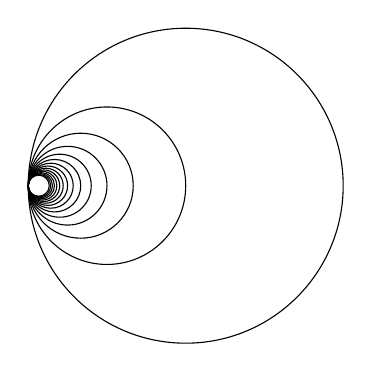
\begin{tikzpicture}
			\def \rad{2}
			\foreach \x in {1,...,15}
			{ \draw (\rad/\x, 0) circle (\rad/\x); }
		\end{tikzpicture}

		A depiction of $\displaystyle\bigcup_{n = 1}^{15}C_n$
	\end{center}

	To see this, consider the point $(0, 0) \in C.$ Given any $\delta > 0,$ there exists $n \in \mathbb{N}$ such that $C_n$ is completely contained in the $\delta$ neighbourhood of $(0, 0).$\\
	Consider the loop $\sigma$ starting at $(0, 0)$ and looping around $C_n$ once. Now, we need to show that $\sigma$ cannot be contracted to a point, \emph{even if we allow the loop to go outside} $U.$\\
	To do this, we consider the map $p:(C, (0, 0)) \to (S^1, (1, 0))$ which maps $C_n$ to $S^1$ in the natural way and collapses maps everything else to $(1, 0).$\\
	(It can be verified that this is a continuous function.)\\
	Now, we see that $p_*:\pi_1(C, (0, 0)) \to \pi_1(S^1, (1, 0))$ maps $[\sigma]$ to the generator of $\pi_1(S^1, (1, 0)).$ In particular, $[\sigma]$ is not trivial (in $C,$ not just in $U$).
\end{ex}

\subsection{Constructing the universal covering space}
\begin{thm}
	If $X$ is a semi-locally simply connected (and path-connected and locally path-connected) space, then $X$ has a universal covering.
\end{thm}
In this subsection, we give a proof of this theorem by constructing a universal covering. We shall fix $X$ to be as in the theorem.\\
%
%
\begin{proof} \phantom{hi}\\
\textsc{Step 1.} \textbf{Constructing the set $\tilde{X}.$}\\
Choose $x_0 \in X.$ We consider the set $S$ all paths in $X$ with initial point $x_0.$ Define $\sim$ on $S$ by $\alpha \sim \beta$ if $\alpha\simeq\beta\rel\{0, 1\}.$ (In particular, $\alpha(1) = \beta(1).$)\\
Let $\langle \alpha\rangle$ be the equivalence class of $\alpha.$ We define
\begin{equation*} 
	\tilde{X} = S/{\sim} = \{\langle \alpha\rangle \mid \alpha \in S\}.
\end{equation*}

\dotfill

\textsc{Step 2.} \textbf{Giving $\tilde{X}$ a topology - defining a basis.}\\
Let $V$ be a neighbourhood of $\alpha(1).$ We define $\langle a, V\rangle$ to be the set of all $\langle \alpha\beta\rangle$ where $\beta$ is a path in $V$ with initial point $\alpha(1).$\\
Let $\mathcal{B}$ be the set of all $\langle \alpha, V\rangle$s. We show that $\mathcal{B}$	is a base.\\
Note that $\langle \alpha\rangle \in \langle \alpha, X\rangle$ and thus, every element of $\tilde{X}$ does indeed belong to an element of $\mathcal{B}.$\\
Now, suppose $\langle \alpha''\rangle \in \langle \alpha, V\rangle \cap \langle \alpha', V'\rangle.$ In particular, $\langle \alpha''\rangle \in \langle \alpha, V\rangle$ which gives that $\alpha''(1) \in V.$ Thus, $V$ is a neighbourhood of $\alpha''(1)$ as well. Moreover, if 
\begin{equation*} 
	\alpha'' \simeq \alpha\beta\rel\{0, 1\}
\end{equation*} 
for some path $\beta$ in $V,$ then 
\begin{equation*} 
	\alpha \simeq \alpha''\beta^{-1}\rel\{0, 1\}
\end{equation*} with $\beta'$ again being in $V.$\\
Thus, we see that $\langle \alpha'', V\rangle = \langle \alpha, V\rangle.$\\
Similarly, $\langle \alpha'', V'\rangle = \langle \alpha', V'\rangle.$ Now,
\begin{equation*} 
	\langle \alpha, V\cap V'\rangle \subset\langle \alpha'', V\rangle\cap\langle \alpha'', V'\rangle
\end{equation*}
or
\begin{equation*} 
	\langle \alpha''\rangle \in \langle \alpha'', V\cap V'\rangle \subset\langle \alpha, V\rangle\cap\langle \alpha', V'\rangle,
\end{equation*}
proving that $\mathcal{B}$ is a basis.\\
Of course, we now give $\tilde{X}$ the topology generated by $\mathcal{B}.$

\dotfill

\textsc{Step 3.} \textbf{Defining the map $p$.}\\
Define
\begin{equation*} 
	p:\tilde{X} \to X
\end{equation*}
as
\begin{equation*} 
	p\langle \alpha\rangle = \alpha(1).
\end{equation*}
(Clearly, this is well-defined.)\\
To show that this is a map, that is, it is continuous, note that given any $\langle \alpha\rangle$ and any open set $V$ containing $\alpha(1),$ the set $p\langle \alpha, V\rangle$ is the path component of $\alpha(1)$ in $V.$ (Note that the path component of $\alpha(1)$ in $V$ is precisely the set of all those points $x$ such that there's a path $\alpha(1) \overset{\beta}{\longrightarrow}x.$ Then, $x = p\langle \alpha\beta\rangle \in p\langle \alpha, V\rangle.$)\\
Thus, given any $\langle \alpha\rangle \in \tilde{X}$ and neighbourhood $V$ of $p\langle \alpha\rangle,$ we have that the neighbourhood $\langle \alpha, V\rangle$ of $\langle \alpha\rangle$ gets mapped in $V.$ This shows that $p$ is continuous. In fact, this also shows that $p$ is open since basis elements get mapped to open sets. (Path components are connected components (since $X$ is locally path-connected) which are open.)

\dotfill

\textsc{Step 4.} \textbf{Showing that $\tilde{X} \overset{p}{\longrightarrow} X$ is a covering map.}\\
Given $x \in X,$ choose a \emph{path-connected} neighbourhood $V$ of $x$ such that any loop at $x$ in $V$ can be shrunk to $x$ in $X.$ (We use the fact that $X$ is locally path-connected and semi-locally simply connected.) \\
We show that $V$ is evenly covered. \\
Let $\alpha$ be any path starting at $x_0$ such that $p\langle \alpha\rangle \in V.$ (Such a path does exist since $X$ is path-connected and so, there exists $x_0\overset{\alpha}{\longrightarrow} x \in V.$) \\
\begin{blockquote}
	\textbf{Claim 1.} $p\langle \alpha, V\rangle = V.$
	\begin{proof} 
		It follows by our previous observation that $p\langle \alpha, V\rangle \subset V.$ We have equality this time since $V$ is path-connected.
	\end{proof}
\end{blockquote}
We show that $p$ maps $\langle \alpha, V\rangle$ homeomorphically onto $V.$\\
Well, we have already shown that it is \emph{onto.} We had also shown that this is continuous and open. Thus, all we need to show that this one-one. For then, it would follow that it is a bijection and that the inverse is also continuous. (By virtue of it being open.)\\
Suppose that $p\langle \alpha\beta\rangle = p\langle \alpha\beta'\rangle.$ (Note that $\langle \alpha\beta\rangle$ is a typical element of $\langle \alpha, V\rangle$ where $\beta$ is a path in $V$ starting at $\alpha(1)$.)\\
Then, $\beta$ and $\beta'$ have the same terminal points (and of course, initial points as well). Note that $\beta\beta'^{-1}$ is a loop at $x.$ By choice of $V,$ we have
\begin{equation*} 
	\beta\beta^{-1} \simeq e_x \rel\{0, 1\}
\end{equation*}
or
\begin{equation*} 
	\alpha\beta \simeq \alpha\beta' \rel\{0, 1\}
\end{equation*}
giving
\begin{equation*} 
	\langle \alpha\beta\rangle = \langle \alpha\beta'\rangle,
\end{equation*}
as desired.\\~\\
Moreover, note that the complete preimage of $V$ is the disjoint union of all $\langle \alpha, V\rangle$ such that $p\langle \alpha\rangle \in V.$ (That this is the complete preimage is obvious.) \\
To see that the union is disjoint, suppose $\alpha$ and $\alpha'$ are paths such that $\langle \alpha, V\rangle \cap \langle \alpha', V\rangle \neq \emptyset.$ Then, for $\langle \alpha''\rangle$ in the intersection, we have
\begin{equation*} 
	\langle \alpha, V\rangle = \langle \alpha'', V\rangle = \langle \alpha', V\rangle,
\end{equation*} 
as earlier, showing that the union is disjoint.\\
Thus, this is the decomposition of $p^{-1}(V)$ into sheets, as desired.

\dotfill

\textsc{Step 5.} \textbf{$\tilde{X}$ is path-connected.}\\
Let $\widetilde{x_0} = \langle e_{x_0}\rangle,$ the class of the constant loop at $x_0.$ We show that we can join any point $\langle \alpha\rangle \in \tilde{X}$ to $\widetilde{x_0}$ which would show that $\tilde{X}$ is path-connected.\\
Given a path $x_0 \overset{\alpha}{\longrightarrow} x$ in $X,$ define
\begin{equation*} 
	\alpha_s(t) = \alpha(st), \quad s, t \in I.
\end{equation*}
Thus, for each $s \in I,$ $\alpha_s$ is a path in $X$ such that $\alpha_s(0) = \alpha(0) = x_0.$ That is, each $\alpha_s$ is a path starting at $x_0.$\\
Now, define $\tilde{\alpha}:I \to \tilde{X}$ as 
\begin{equation*} 
	\tilde{\alpha}(s) := \langle \alpha_s\rangle.
\end{equation*}
Note that $\alpha_0$ is the constant loop at $x_0$ and $\alpha_1 = \alpha.$ Thus, we have that 
\begin{equation*} 
	\widetilde{x_0} \overset{\tilde{\alpha}}{\longrightarrow} \langle \alpha\rangle
\end{equation*}
is a path in $\tilde{X},$ provided we show that $\tilde{\alpha}$ is continuous.\\
To see this, let $s_0 \in I$ be arbitrary and consider a basis neighbourhood $\langle \alpha_{s_0}, V\rangle$ of $\tilde{\alpha}(s) = \alpha_s.$\\
Note that $\alpha_{s_0}(1) \in V,$ that is, $\alpha(s_0) \in V.$ Since $\alpha$ is continuous, there exists a $\delta$-neighbourhood $U$ around $s_0$ such that $\alpha(U) \subset V.$\\
We show that $\tilde{\alpha}(U) \subset \langle \alpha_{s_0}, V\rangle.$\\
To see this, let $s \in U.$ Then,
\begin{equation*} 
	p\langle \alpha_s\rangle = \alpha_s(1) = \alpha(s) \in V.
\end{equation*}
Let $s_M = \max\{s, s_0\}$ and $s_m = \min\{s, s_0\}.$ \\
Then, note that the $\alpha_{s_M}$ is a path which can be seen as a product of the path $\alpha_{s_m}$ with a path joining the point $\alpha(s_m)$ to $\alpha(s_M),$ the latter lying completely in $V$ since $\alpha(U) \subset V.$\\
Thus, we see that $\langle \alpha_{s_M}\rangle \in \langle \alpha_{s_m}, V\rangle$ and vice-versa. Since $\{s_m, s_M\} = \{s, s_0\},$ we see that
\begin{equation*} 
	\tilde{\alpha}(s) = \langle \alpha_s\rangle \in \langle \alpha_{s_0}, V\rangle,
\end{equation*}
as desired. This shows that $\tilde{\alpha}$ is continuous and thus, $\tilde{X}$ is path connected.\\
Moreover, we see that
\begin{equation*} 
	(p\circ\tilde{\alpha})(s) = p\langle \alpha_s\rangle = \alpha_s(1) = \alpha(s),
\end{equation*}
that is, $\tilde{\alpha}$ lifts $\alpha.$ 

\dotfill

\textsc{Step 6.} \textbf{$X$ is simply connected.}\\
We show that $\pi_1(\tilde{X}, \widetilde{x_0})$ is trivial.\\
Let $\tau$ be a loop in $\tilde{X}$ at $\widetilde{x_0},$ and let $\alpha = p \circ \tau.$ By uniqueness of lifts, we have
\begin{equation*} 
	\tau = \tilde{\alpha},
\end{equation*}
where $\tilde{\alpha}$ is defined as earlier. (Uniqueness since both $\tau$ and $\tilde{\alpha}$ have initial point $\widetilde{x_0}.$) \\
In particular, $\tilde{\alpha}$ is a loop at $\widetilde{x_0}$ (since so was $\tau$).\\
Thus, we have
\begin{equation*} 
	\langle \alpha\rangle = \langle \alpha_1\rangle = \tilde{\alpha}(1) = \widetilde{x_0} = \langle e_{x_0}\rangle.	
\end{equation*}
(The last equality was the definition of $\widetilde{x_0}.$)\\
Thus, we have
\begin{equation*} 
	\langle \alpha\rangle = \langle e_{x_0}\rangle
\end{equation*}
or that
\begin{equation*} 
	\alpha \simeq e_{x_0} \rel \{0, 1\}.
\end{equation*}
By the \nameref{thm:pathhomotlifts}, we see that 
\begin{equation*} 
	\tilde{\alpha} \simeq \widetilde{e_{x_0}} \rel\{0, 1\}.
\end{equation*}
Since we have $\tilde{\alpha} = \tau$ and $\widetilde{e_{x_0}} = e_{\widetilde{x_0}},$ we are done!
\end{proof}

\hrulefill

The above then finishes our construction as we have shown that
\begin{equation*} 
	(\tilde{X}, \widetilde{x_0}) \overset{p}{\longrightarrow} (X, x_0)
\end{equation*}
is a covering space where $X$ is simply connected.

\begin{cor}
	Under the same hypothesis, for every subgroup $H$ of $\pi_1(X, x_0),$ there exists a covering space $(E, e_0) \overset{p}{\longrightarrow} (X, x_0),$ unique up to equivalence, such that $H = p_*\pi_1(E, e_0).$
\end{cor}
\begin{proof} 
	Let $\tilde{X} \overset{f}{\longrightarrow} X$ be the universal covering space, $G$ its group of covering transformations. By \cref{thm:covtransiso}, $G \cong \pi_1(X, x_0).$ Let $H' \le G$ be the subgroup corresponding to $H.$ \\
	\begin{blockquote}
	Note that $H'$ must act evenly. \\
	To see this, let $\tilde{x} \in \tilde{X}.$ Let $U$ be an evenly covered neighbourhood of $p(\tilde{x})$ and let $\{S_i\}$ be sheets over $U.$ Let $S_{i_0}$ be the sheet containing $\tilde{x}.$ Let $\varphi \in H'.$ Since $f\varphi = f,$ we see that $f$ maps $S = \bigsqcup S_i$ onto itself. Since the sheets are the path-components of $S,$ we see that sheets are mapped onto sheets. Moreover, note
	\begin{equation*} 
		S_{i_0} = f(S_{i_0}) \implies \varphi = \id_{\tilde{X}}.
	\end{equation*}
	(This follows at once from \nameref{thm:uniquelift}. (Since $\varphi$ and $\id_{\tilde{X}}$ are lifts of $f$.))\\
	Thus, if $\varphi \neq \id_{\tilde{X}},$ we see that $S_{i_0} \cap \varphi(S_{i_0}),$ showing that $H'$ acts evenly.
	\end{blockquote}
\end{proof}

We will now prove a result about topological groups, before which we prove a lemma.

\begin{lem} 
	Let $X$ be a topological group with operation $\cdot$ and identity element $x_0.$ Let $\Omega(X, x_0)$ denote the set of all loops at $x_0$ in $X.$ If $f, g \in \Omega(X, x_0),$ we define a loop $f\otimes g$ at $x_0$ by the rule
	\begin{equation*} 
		(f \otimes g)(s) = f(s)\cdot g(s).
	\end{equation*}
	\begin{enumerate}
		\item This operation makes $\Omega(X, x_0)$ into a group.
		\item This operation induces a group operation $\otimes$ on $\pi_1(X, x_0).$
		\item The two group operations $*$ and $\otimes$ on $\pi_1(X, x_0)$ are the same. (Recall that $*$ was the usual product of paths, in this case, loops.)
		\item $\pi_1(X, x_0)$ is abelian.
	\end{enumerate}
\end{lem}
\begin{proof} 
	\phantom{Hi}
	\begin{enumerate}
		\item This is a simple check. $\otimes$ is associative since $\cdot$ is. Moreover, $e_{x_0},$ the constant loop at $x_0$ acts as the identity as can be easily checked.\\
		Lastly, given $f\in\Omega(X, x_0),$ we see that $g:I\to X$ defined as
		\begin{equation*} 
			g(s) = (f(s))^{-1}
		\end{equation*}
		is an element of $\Omega(X, x_0)$ and is the (two-sided) inverse of $f$ with respect to $\otimes.$\\
		Thus, $\Omega(X, x_0)$ is a group under $\otimes.$
		\item In other words, we need to show that if $f \simeq f'$ and $g \simeq g',$ both $\rel \{0, 1\},$ then
		\begin{equation*} 
			f\otimes g \simeq f'\otimes g' \rel\{0, 1\}.
		\end{equation*}
		To see this, let $H:f\simeq f' \rel\{0, 1\}$ and $H':g\simeq g'\rel\{0, 1\}$ be path homotopies. We define a new path homotopy 
		\begin{equation*} 
			H\otimes H': I \times I \to X
		\end{equation*} given as
		\begin{equation*} 
			(H \otimes H')(s, t) = H(s, t)\cdot H'(s, t).
		\end{equation*}
		One can note that $(H\otimes H')(0, t) = x_0\cdot x_0$ and similarly for $(1, t).$\\
		Likewise, we have 
		\begin{equation*} 
			(H \otimes H')(s, 0) = H(s, 0)\cdot H'(s, 0) = f(s)\cdot g(s) = (f\otimes g)(s)
		\end{equation*}
		and similarly for $(s, 1).$\\
		This shows that $\otimes$ induces a group operation on $\pi_1(X, x_0).$ 
		\item To do this and the next part, we just show that
		\begin{equation*} 
			([f] \otimes [g]) * ([\sigma] \otimes [\tau]) = ([f] * [\sigma]) \otimes ([g] * [\tau])
		\end{equation*}
		for all $f, g, \sigma, \tau \in \Omega(X, x_0).$ The result will then follow from \nameref{thm:eckmannhilton}.\\
		Since both $*$ and $\star$ are compatible with $[\cdot],$ the above is equivalent to
		\begin{equation*} 
			[\underbrace{(f \otimes g)*(\sigma \otimes \tau)}_{=\vcentcolon \alpha}] = [\underbrace{(f * \sigma) \otimes (g * \tau)}_{=\vcentcolon\beta}].
		\end{equation*}
		Thus, if we show that $\alpha \simeq \beta \rel \{0, 1\},$ then we are done. In fact, we will show that $\alpha = \beta.$\\
		Indeed, we have
		\begin{align*} 
			\alpha(s) &= \left((f \otimes g)*(\sigma \otimes \tau)\right)(s)\\
			&= \begin{cases}
				(f\otimes g)(2s) & 0 \le 2s \le 1,\\
				(\sigma \otimes \tau)(2s - 1) & 1 \le 2s \le 2
			\end{cases}\\
			&= \begin{cases}
				f(2s)\cdot g(2s) & 0 \le 2s \le 1,\\
				\sigma(2s - 1)\cdot\tau(2s - 1) & 1 \le 2s \le 2.
			\end{cases}
		\end{align*}
		On the other hand, we have
		\begin{align*} 
			\beta(s) &= \left((f * \sigma) \otimes (g * \tau)\right)(s)\\
			&= \left((f*\sigma)(s)\right)\cdot\left((g*\tau)(s)\right)\\
			&= \begin{cases}
				f(2s)\cdot g(2s) & 0 \le 2s \le 1,\\
				\sigma(2s - 1)\cdot\tau(2s - 1) & 1 \le 2s \le 2.
			\end{cases}
		\end{align*}
		Thus, we see that $\alpha = \beta,$ as desired. \qedhere
	\end{enumerate}
\end{proof}

\begin{thm}
	If $X$ is a topological group with operation $\cdot$, then for any covering space $E \overset{p}{\longrightarrow} X$ and point $e_0$ in the fiber of the neutral element $x_0$ of $X,$ there is a unique structure of topological group on $E$ for which $e_0$ is the neutral element and $p$ is a homomorphism.
\end{thm}
\begin{proof} 
	Let $m:X\times X \to X$ be the map $(x_1, x_2) \mapsto x_1\cdot x_2^{-1}.$ We wish to lift the red map $m\circ(p \times p)$ to a map $m'$ as shown.
	\begin{center}
		\begin{tikzcd}
		{(E \times E, (e_0, e_0))} \arrow[dd, "p\times p"', red] \arrow[rr, "m'", dashed] &  & {(E, e_0)} \arrow[dd, "p"] \\ &  & \\
		{(X \times X, (x_0, x_0))} \arrow[rr, "m"', red]&  & {(X, x_0)}                
		\end{tikzcd}
	\end{center}
	Once we do that, we would define $\cdot$ on $E$ induced by $e_1\cdot e_2^{-1} = m'(e_1, e_2).$ \\
	Note that any other structure would also make the above diagram commute (since $p$ is a homomorphism) and thus, $m'$ (if it exists) is unique. (By \nameref{thm:uniquelift}.)\\
	The criterion for its existence is 
	\begin{equation*} 
		m_*(p \times p)_*\pi_1(E \times E, (e_0, e_0)) \subset p_*\pi_1(E, e_0),
	\end{equation*}
	as given by \cref{thm:liftcriterion}.\\
	Let us first examine $m_*.$ Given $[\alpha] \in \pi_1(X\times X, (x_0, x_0)),$ we have
	\begin{equation*} 
		m_*([\alpha]) = [m \circ \alpha].
	\end{equation*}
	Note that any loop $\alpha$ at $(x_0, x_0)$ in $X \times X$ looks like
	\begin{equation*} 
		\alpha = \alpha_1 \times \alpha_2
	\end{equation*}
	for some loops $\alpha_1$ and $\alpha_2$ at $x_0$ in $X.$ Thus, we have
	\begin{equation*} 
		(m\circ\alpha)(t) = \alpha_1(t)\cdot(\alpha_2(t))^{-1}, \quad t \in I.	
	\end{equation*}
	By the previous lemma, we conclude that
	\begin{equation*} 
		m\circ\alpha = \alpha_1*\alpha_2^{-1},
	\end{equation*}
	where the $*$ and $^{-1}$ are the usual path (in this case, loop) operations.\\
	Similarly, if $\sigma$ is a loop at $(e_0, e_0)$ in $E \times E,$ then $\sigma = (\sigma_1, \sigma_2)$ for some loops $\sigma_1, \sigma_2$ at $e_0$ in $E.$ Moreover, we have
	\begin{align*} 
		(p\times p)\circ\sigma = (p \circ \sigma_1)\times(p \circ \sigma_2).
	\end{align*}
	Thus,
	\begin{align*} 
		m\circ(p \times p) \circ \sigma &= (p \circ \sigma_1)*(p \circ \sigma_2)^{-1}\\
		&= p \circ (\sigma_1 * \sigma_2^{-1})
	\end{align*}
	or
	\begin{equation*} 
		m_*(p\times p)_*[\sigma] = p_*[\sigma_1 * \sigma_2^{-1}],	
	\end{equation*}
	showing that
	\begin{equation*} 
		m_*(p \times p)_*\pi_1(E\times E, (e_0, e_0)) \subset p_*(E_1, e_0),
	\end{equation*}
	fulfilling the lifting criterion.\\~\\
	Thus, the lift $m'$ exists. We now show that it gives $E$ the structure of a topological group such that $e_0$ is the neutral element and $p$ is homomorphism.
\end{proof}
\end{document}